
\section*{Testiranje strelske metode}

Kot prvo sem preizkusil enodimenzijski linearni strelski problem - vodoravni met, kjer je znano, da je $v_{0y}=0$. Določil sem domet izstrelka $x(t_{max})=L$ in streljal s parametrom $v_{0x}$, pri čemer sem uporabljal metodo za ekstrapolacijo rešitve iz dvoje strelov:
\begin{equation}
    y(x) = (1-\theta)\,y_1(x)+\theta\,y_2(x), \quad \theta = \frac{L-x_1(t_{max})}{x_2(t_{max})-x_1(t_{max})}.
\end{equation}

Sprostil sem še parameter $v_{0y}$ in preizkusil obe metodi, strelsko in v scipy implementirano kolokacijsko metodo v solve\_bvp na primeru poševnega meta iz izhodišča.

\begin{figure}[h]
    \centering
    \begin{subfigure}{.49\textwidth}
        \centering
        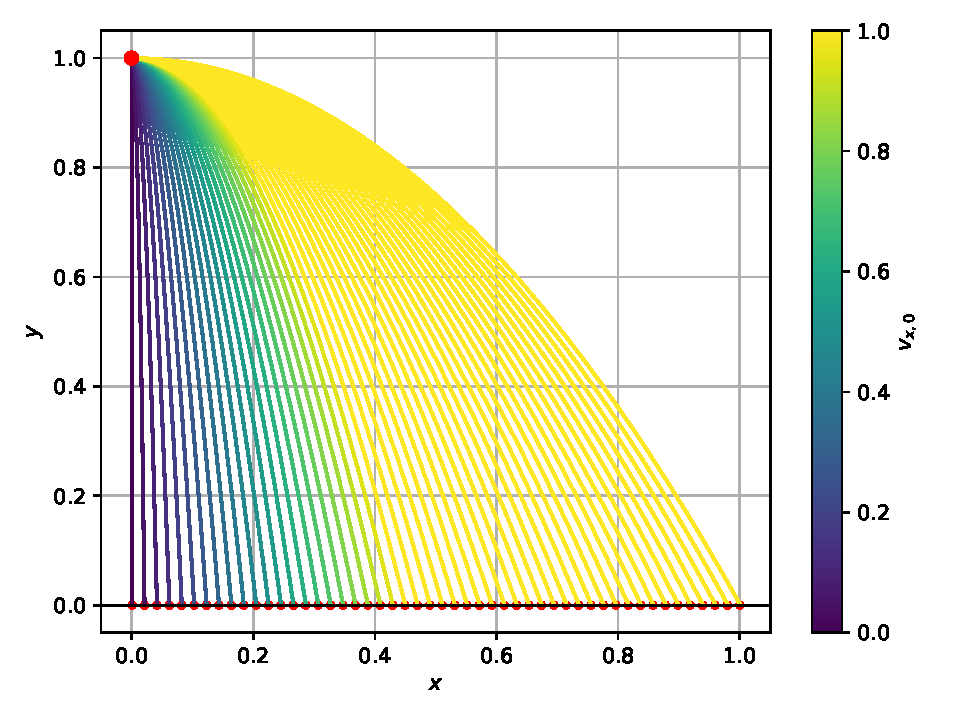
\includegraphics[width=\linewidth]{2.nal_slike/vodoravni.pdf}
        \caption{različne rešitve strelske metode za vodoravni met}
    \end{subfigure}
    \begin{subfigure}{.49\textwidth}
        \centering
        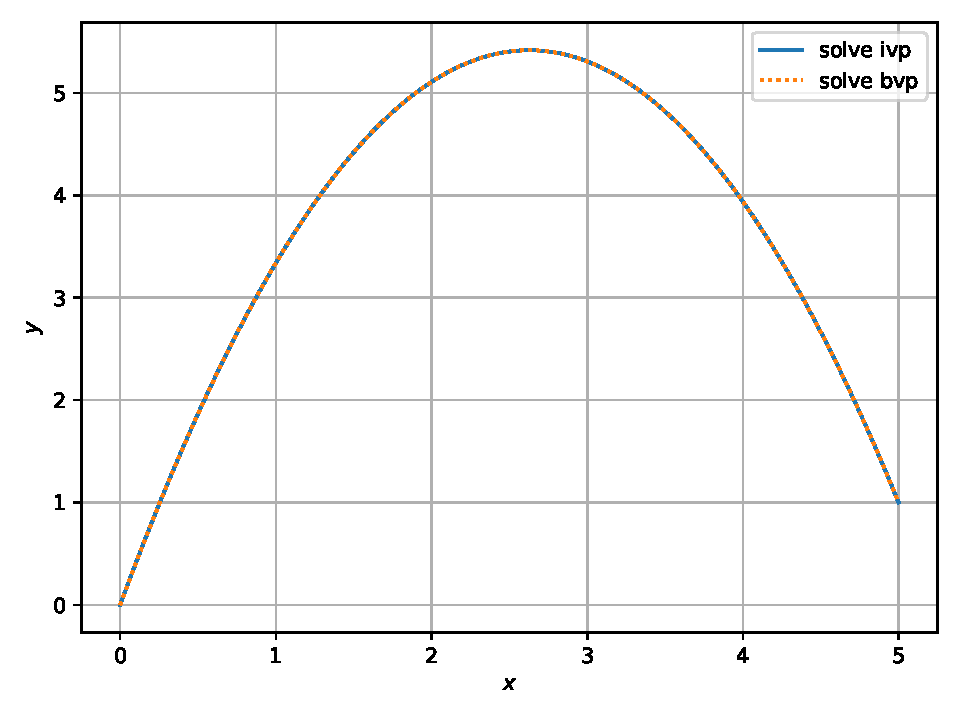
\includegraphics[width=\linewidth]{2.nal_slike/posevni_met.pdf}
        \caption{rešitev za poševni met do točke (5,1)}
    \end{subfigure}
    \caption{}
\end{figure}

\section{Vrteča vrv}

Obravnavamo sistem DE v brezdimenzijski obliki:
\begin{equation}
    \begin{aligned}
        \frac{dF}{ds} &= \sin\alpha - \beta \times \cos\alpha \\
        \frac{d\alpha}{ds} &= \frac{1}{F}\,(\cos\alpha + \beta\times\sin\alpha)\\
        \frac{dx}{ds} &= \cos\alpha\\
        \frac{dy}{ds} &= \sin\alpha,
    \end{aligned}
\end{equation}
kjer je $F$ sila v vrvi, $\alpha$ naklon vrvi in $x,y$ lega vrvi. $\beta$ je parameter, ki opisuje hitrost vrtenja, poznamo začetno lego $(x_0,y_0)=(0,0)$ in končno $(x_f,y_f)=(0,y_f)$, kjer lahko določamo razdaljo med krajišči. Pri tem streljamo $F_0$ in $\alpha_0$, da zadenemo ciljno lego.

Nekaj izmed vseh mnogih rešitev je prikazano na spodnji sliki. Opazimo, da večanje $\beta$ povzoroča več `vozlov', torej točk, ko vrv preseka ravnovesno lego. Obstaja pa takšen $\beta$, ko je vrv popolnoma napeta. Pri majhnih $y_f$ in velikih $\beta$ prihaja do nihanja vrvi pod ciljno lego, kjer le-ta večkrat veka samo sebe, kar bi pri eksperimentu zagotovo povzročalo težave, zato takšne rešive po mojem mnenju niso mogoče in bi v tem primeru bilo potrebno nadgraditi model!

\begin{figure}[h]
    \centering
    \begin{subfigure}{.49\textwidth}
        \centering
        \includegraphics[width=\linewidth]{2.nal_slike/vrv_yf_0.3.pdf}
        \caption{$y_f=0,3$}
    \end{subfigure}
    \begin{subfigure}{.49\textwidth}
        \centering
        \includegraphics[width=\linewidth]{2.nal_slike/vrv_yf_0.4.pdf}
        \caption{$y_f=0,4$}
    \end{subfigure}
    \begin{subfigure}{.49\textwidth}
        \centering
        \includegraphics[width=\linewidth]{2.nal_slike/vrv_yf_0.5.pdf}
        \caption{$y_f=0,5$}
    \end{subfigure}
    \begin{subfigure}{.49\textwidth}
        \centering
        \includegraphics[width=\linewidth]{2.nal_slike/vrv_yf_0.6.pdf}
        \caption{$y_f=0,6$}
    \end{subfigure}
    \begin{subfigure}{.49\textwidth}
        \centering
        \includegraphics[width=\linewidth]{2.nal_slike/vrv_yf_0.9.pdf}
        \caption{$y_f=0,9$}
    \end{subfigure}
    \caption{Različne rešitve glede na končno lego vrvi $y_f$ in parameter $\beta$}
\end{figure}

Ker se je v prejšnji nalogi presenetljivo dobro izkazala lastna implementacija integratorja Runge Kutta 4.reda, ga bom v tem poglavju ponovno uporabljal, saj se izkaže za dovolj hitrega in natančnega, čeprav uporablja konstanten korak, saj so stvari dovolj pohlevne.

\begin{figure}[H]
    \centering
    \begin{subfigure}{.49\textwidth}
        \centering
        \includegraphics[width=\linewidth]{2.nal_slike/F_vrv_yf_0.5.pdf}
        \caption{$y_f=0,6$}
    \end{subfigure}
    \begin{subfigure}{.49\textwidth}
        \centering
        \includegraphics[width=\linewidth]{2.nal_slike/F_vrv_yf_0.9.pdf}
        \caption{$y_f=0,9$}
    \end{subfigure}
    \caption{Potek (normirane) sile po vrvi}
\end{figure}

Za $\beta=100$ in $y_f=0,5$ sem izvedel tudi iskanje rešitve po principu \textit{grid-search}, kjer lepo vidimo območja, kjer se približamo robnim pogojem. To so prave rešitve problema.

\begin{figure}[h]
    \centering
    \includegraphics[width=0.75\linewidth]{2.nal_slike/2d_napaka_ZP_yf_0.5.pdf}
    \caption{Napaka izpoljenvanja robnega pogoja na koncu vrvi v odvisnosti od začetnih pogojev strejljanja}
\end{figure}

Dalje sem analiziral, kako natančno se pri strelski metodi izpolnijo robni pogoji. Uporabil sem funkcijo \texttt{root} it scipy.optimize in računal napako glede na željeno končno lego. Ugotovil sem, da je rezultat dovolj točen, na nivolu numerične napake, nepojasnjeni so le nekateri skoki napake, ki pa so povečini pri majhnih $\beta$. $ds$ predstavlja korak integracije.

Tukaj velja tudi poudariti, da je računanje občutno hitrejše, če se poslužujem preprostega trika pri začetnem približku za iskanje ničle: zanj sem uporabil kar rezultat (ničlo) iz prejšnejga koraka!

Na enak princip sem določil tudi dolžino vrvi in njeno napako od predpisane $L=1$. Napaka je pričakovana že zaradi integratorja (Runge Kutta 4.reda) in je reda velikosti -3. Bolj presenetljivo je, da napaka narašča in nato hitro pade, kar pa tudi zavisi od razdalje med krajiščema; najbolje se obnese pri $y_f/L=0,5$.

\begin{figure}[H]
    \centering
    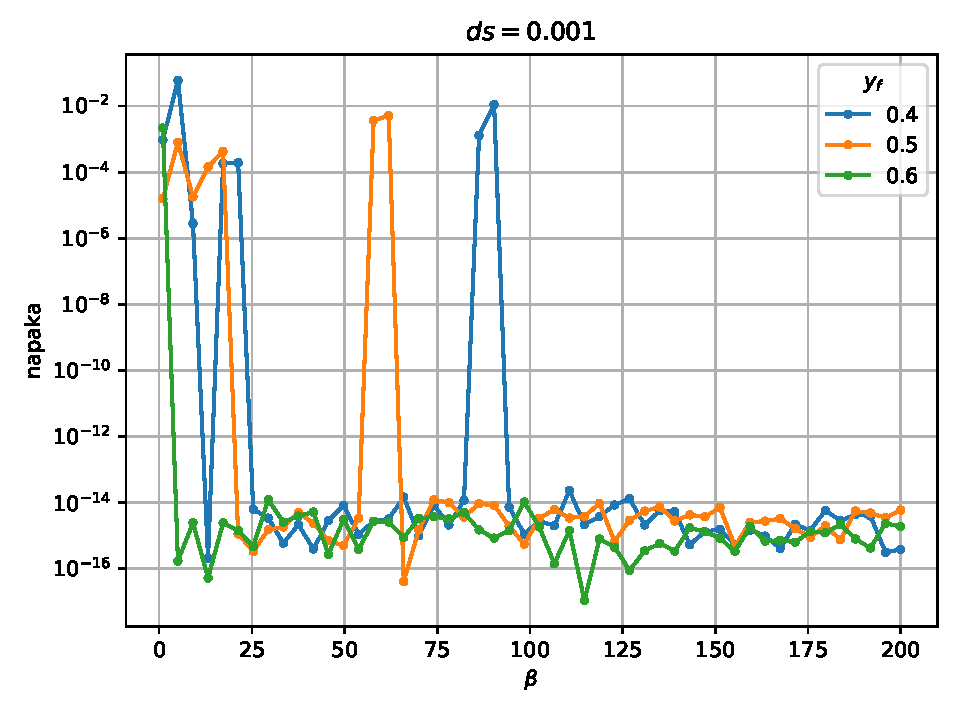
\includegraphics[width=0.6\linewidth]{2.nal_slike/napaka_rp.pdf}
    \caption{Napaka izpoljenvanja robnega pogoja na koncu vrvi}
\end{figure}
\begin{figure}[h]
    \centering
    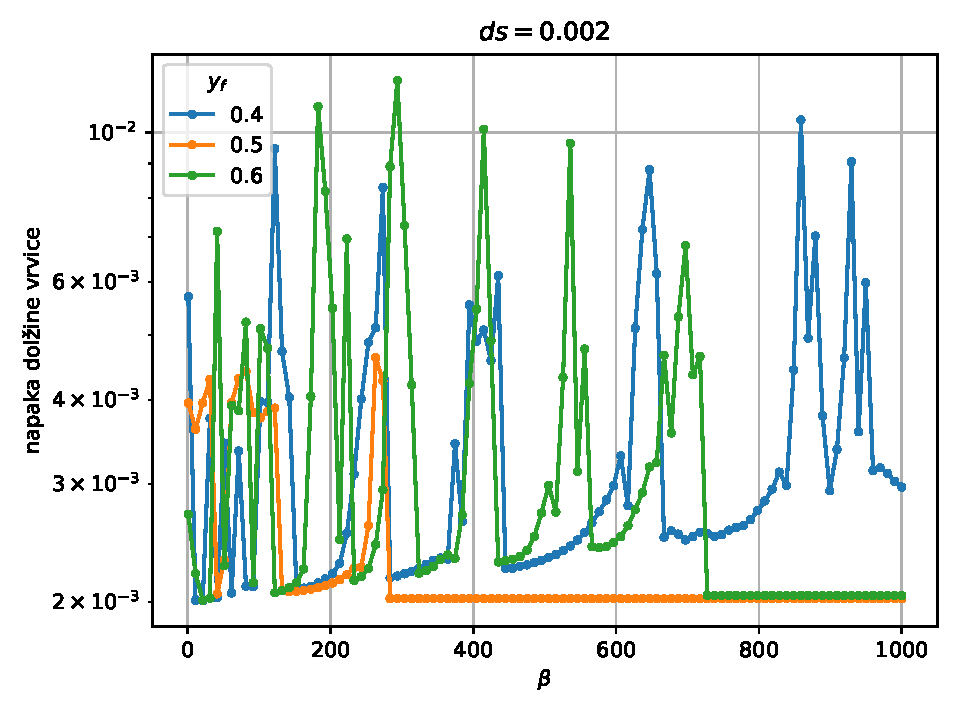
\includegraphics[width=0.6\linewidth]{2.nal_slike/napaka_dolzine.pdf}
    \caption{Napaka izpoljenvanja željene dolžine vrvi}
\end{figure}

\section{Hénon-Heiles potencial}

Podan je Hénon-Heiles potencial:
\begin{equation}
    U(x,y)= \frac{1}{2}\,(x^2+y^2) + x^2\,y - \frac{1}{3}\,y^3,
\end{equation}
ki je trikrat simetričen, zato se lahko za opazovanje periodičosti trajektorij omejim le na začetne lege pri $x_0=0$ in $y_0 \in [0,1]$. Določim tudi začetne hitrosti v x in y smeri, s katerima želim doseči periodične orbite. Pri tem si pomagam z energijo sistema
\begin{equation}
    E(x,y, \dot x, \dot y) = U(x,y) + \frac{1}{2}\,(v_{x}^2+v_{y}^2),
\end{equation}
ki se mora v času ohranjati in jo definiram na začetku simulacije. V splošnem so stabilne trajektorije z $E\leq \frac{1}{6}$.


V takem potencialu zadeve niso več tako pohlevne kot v navadnem (gravitacijskem) potencialu, zato bom uporabljal integratorje v \texttt{scipy.integrate.solve\_ivp}, ki imajo adaptiven časovni korak.

\begin{figure}[ht!]
    \centering
    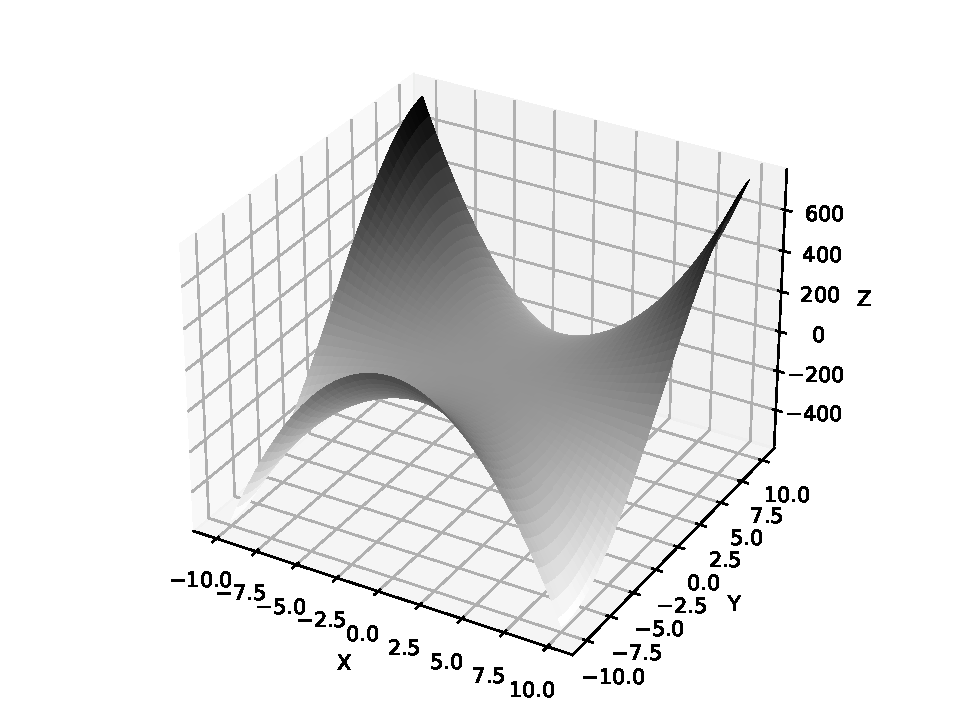
\includegraphics[width=0.7\linewidth]{2.nal_slike/potencial.pdf}
    \caption{Hénon-Heiles potencial}
\end{figure}

\begin{figure}[H]
    \centering
    \begin{subfigure}{.49\textwidth}
        \centering
        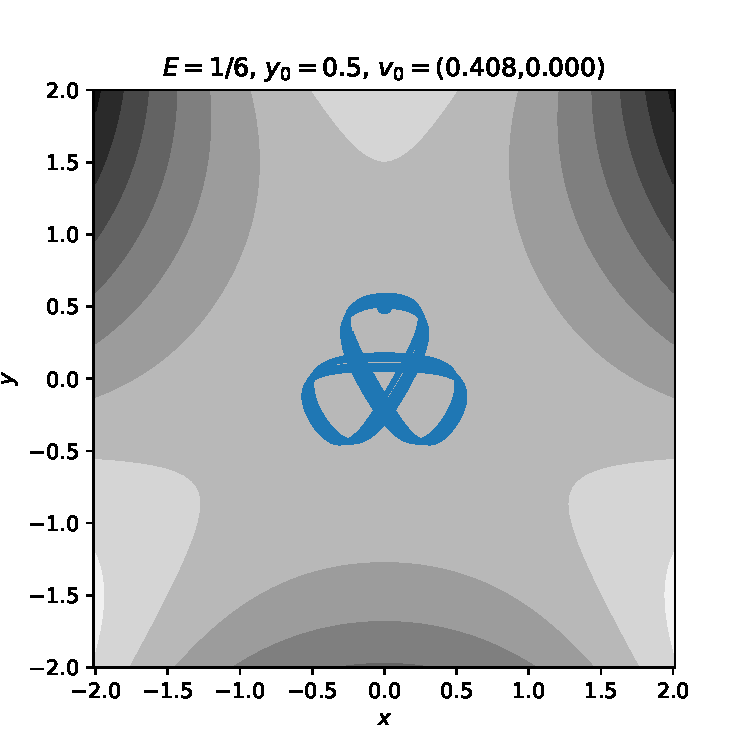
\includegraphics[width=\linewidth]{2.nal_slike/primer1.pdf}
        \caption{primer 1}
    \end{subfigure}
    \begin{subfigure}{.49\textwidth}
        \centering
        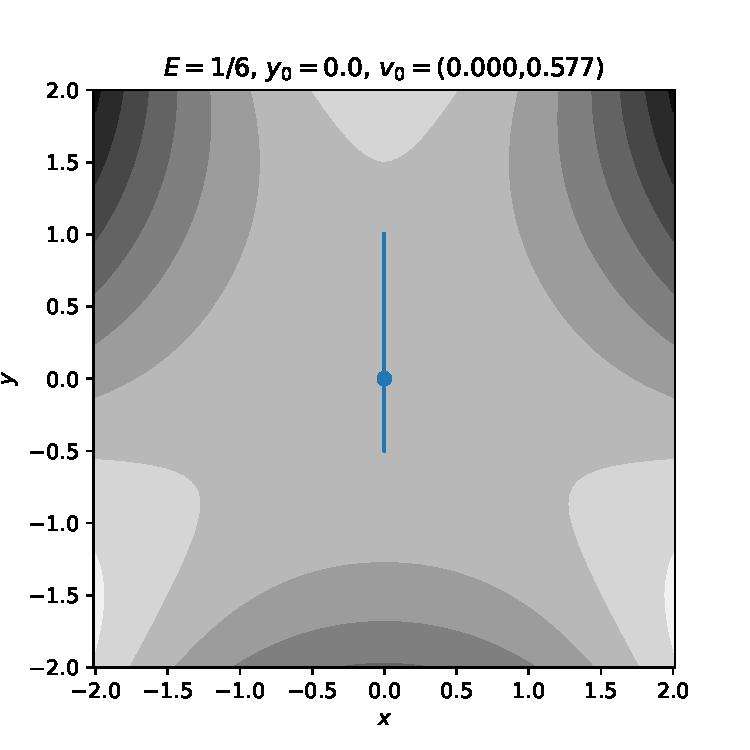
\includegraphics[width=\linewidth]{2.nal_slike/primer2.pdf}
        \caption{primer 2}
    \end{subfigure}
    \begin{subfigure}{.49\textwidth}
        \centering
        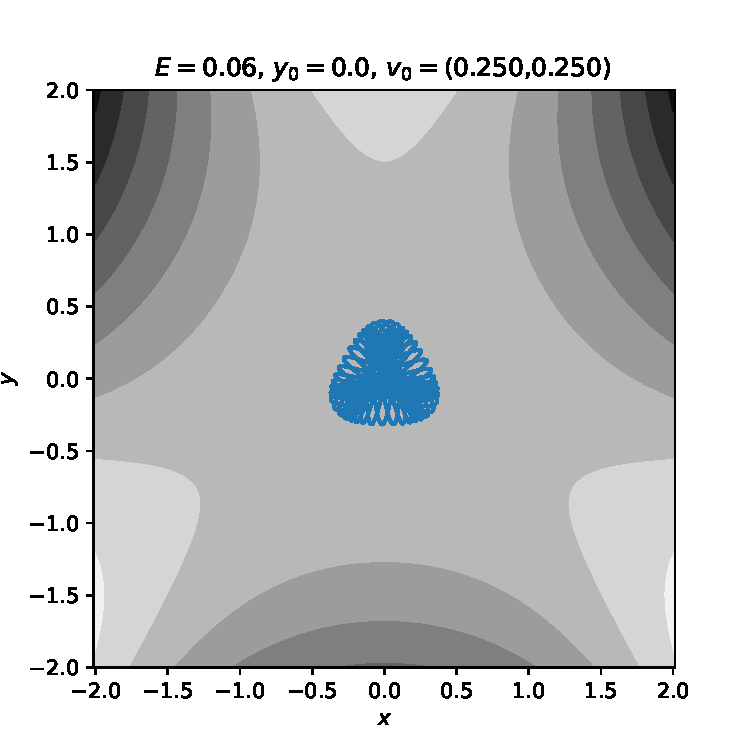
\includegraphics[width=\linewidth]{2.nal_slike/primer3.pdf}
        \caption{primer 3}
    \end{subfigure}
    \begin{subfigure}{.49\textwidth}
        \centering
        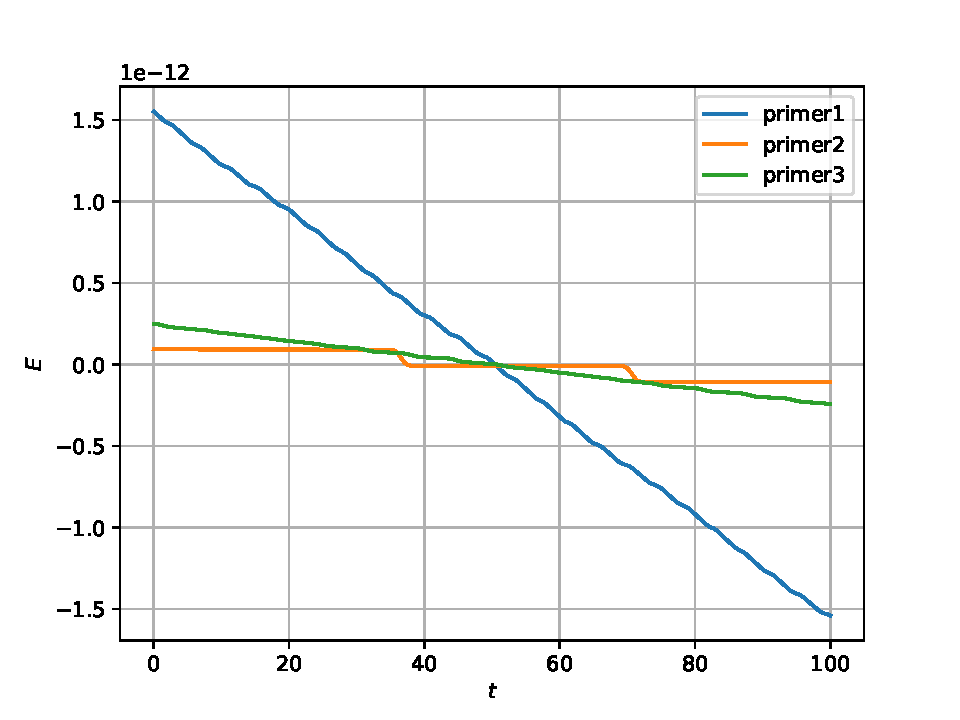
\includegraphics[width=\linewidth]{2.nal_slike/energija_primeri.pdf}
        \caption{ohranjanje energije}
    \end{subfigure}
    \caption{Primeri gibanja v potencialu in potek energije pri integraciji v času}
\end{figure}

Zgoraj so prikazane tri `na oko' periodične orbite, dobljene z ročnim nastavljanjem parametrov. Opazim, da se energija pri integraciji z zadosti majhnim časovnim korakom ohranja, sprememba je reda velikosti numerične napake.

Na spodnji sliki sem streljal pod kotom $\frac{\pi}{4}$ z začetno hitrostjo $\sqrt{2} \,v_0$ in opazoval Poincaréjeve preseke. Tako opazim, da so orbite z nižjimi energijami periodične, pri višjih neperiodične, a še vedno stabilne in pri $E>1/6$ nestabilne. Območje lege se tudi širi iz kroga v trikotnik in nazadnje v pobeg po `dolini' potenciala.

\begin{figure}[h]
    \centering
    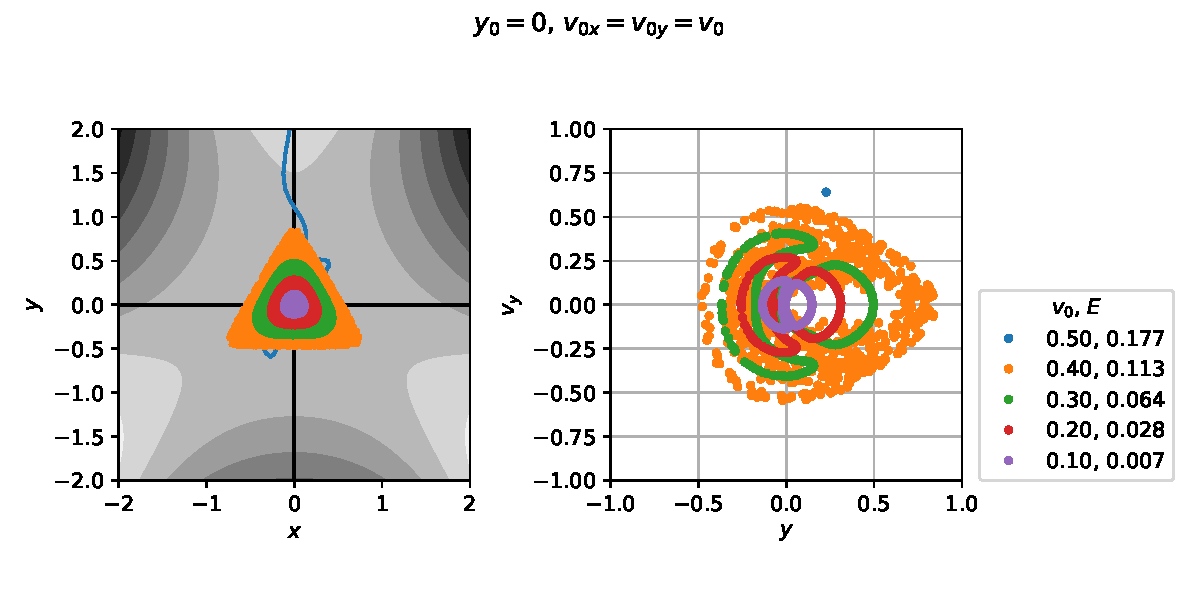
\includegraphics[width=\linewidth]{2.nal_slike/poincare_razlicne_v0.pdf}
    \caption{Orbite z različnimi $v_0$}
\end{figure}

V sledečih slikah so prikazani Poincaréjevi preseki streljanju iz $y_0\in [0,1]$ in pripadajočo $v_{0x}$, da je energija taka, kot je definirana. Pri tem je $v_{0y}=0$. Lege, kjer je potencial večji od dovoljene energije so izpuščene. Pri nižjih energijah je opazno periodično gibanje, ki nato prehaja v neperiodično, a stabilno, kjer je še vedno moč opaziti periodična območja in nazadnje v popolnoma nestabilno. Zanimivo je, da je tudi pri $E\geq 1/6$ moč opaziti periodična območja, vendar ne več dolgo. Z večanjem energije se tudi širi območje lege trajektorij in presečnih leg ter hitrosti.

\begin{figure}[H]
    \centering
    \begin{subfigure}{0.49\textwidth}
        \centering
        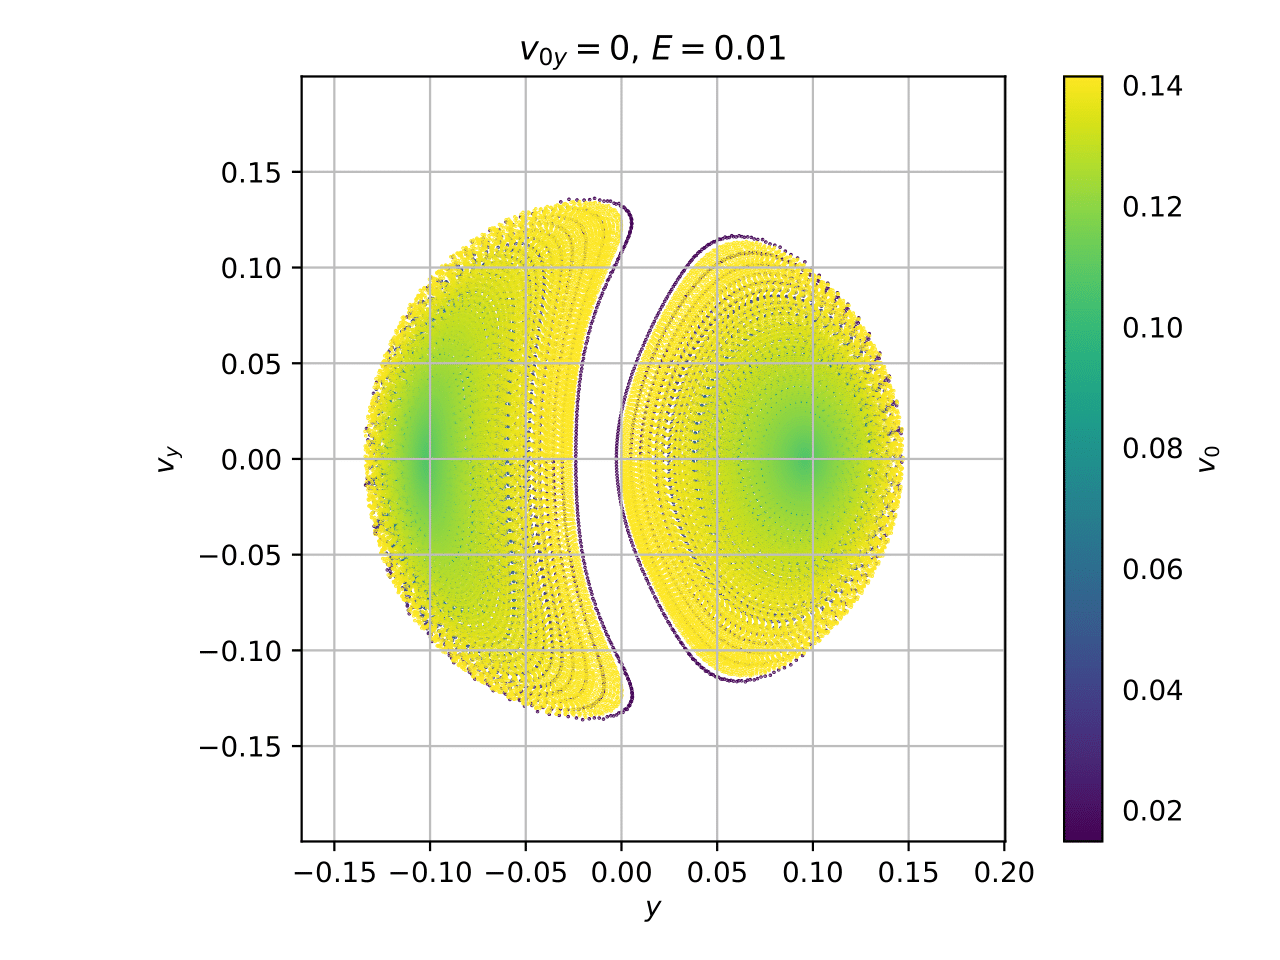
\includegraphics[width=\linewidth]{2.nal_slike/le_v0x/poincare_v0x_E0.01-1.png}
    \end{subfigure}
    \begin{subfigure}{0.49\textwidth}
        \centering
        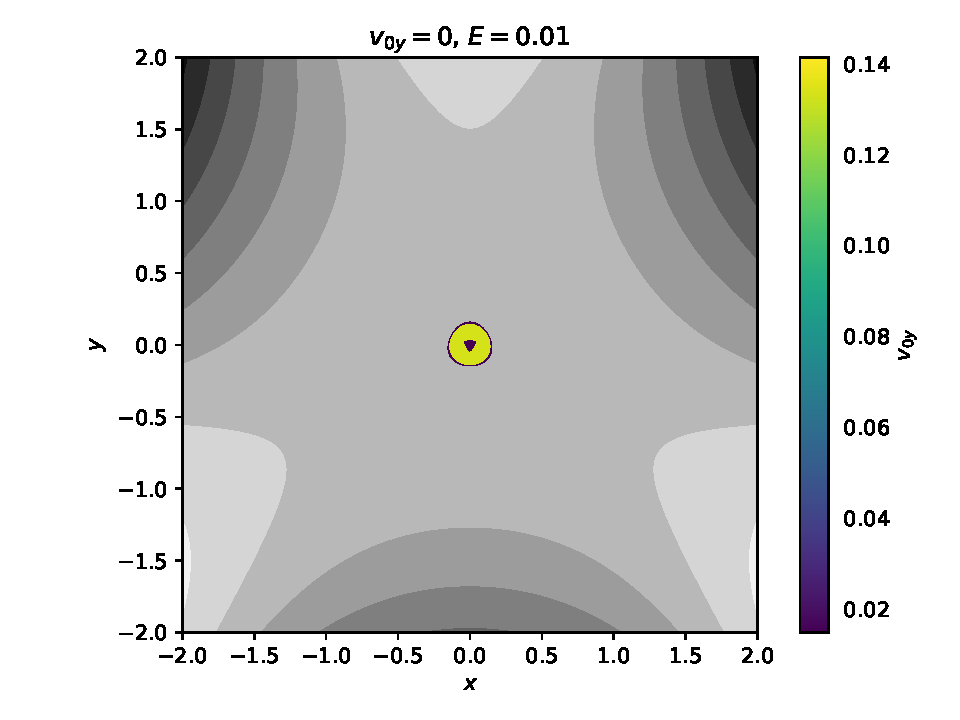
\includegraphics[width=\linewidth]{2.nal_slike/le_v0x/poincare_tajektorije_v0y_E0.01.pdf}
    \end{subfigure}
    \caption{Levo Poincaréjev presek, desno trajktorije pri $E=0,01$}
\end{figure}

\begin{figure}[H]
    \centering
    \begin{subfigure}{0.49\textwidth}
        \centering
        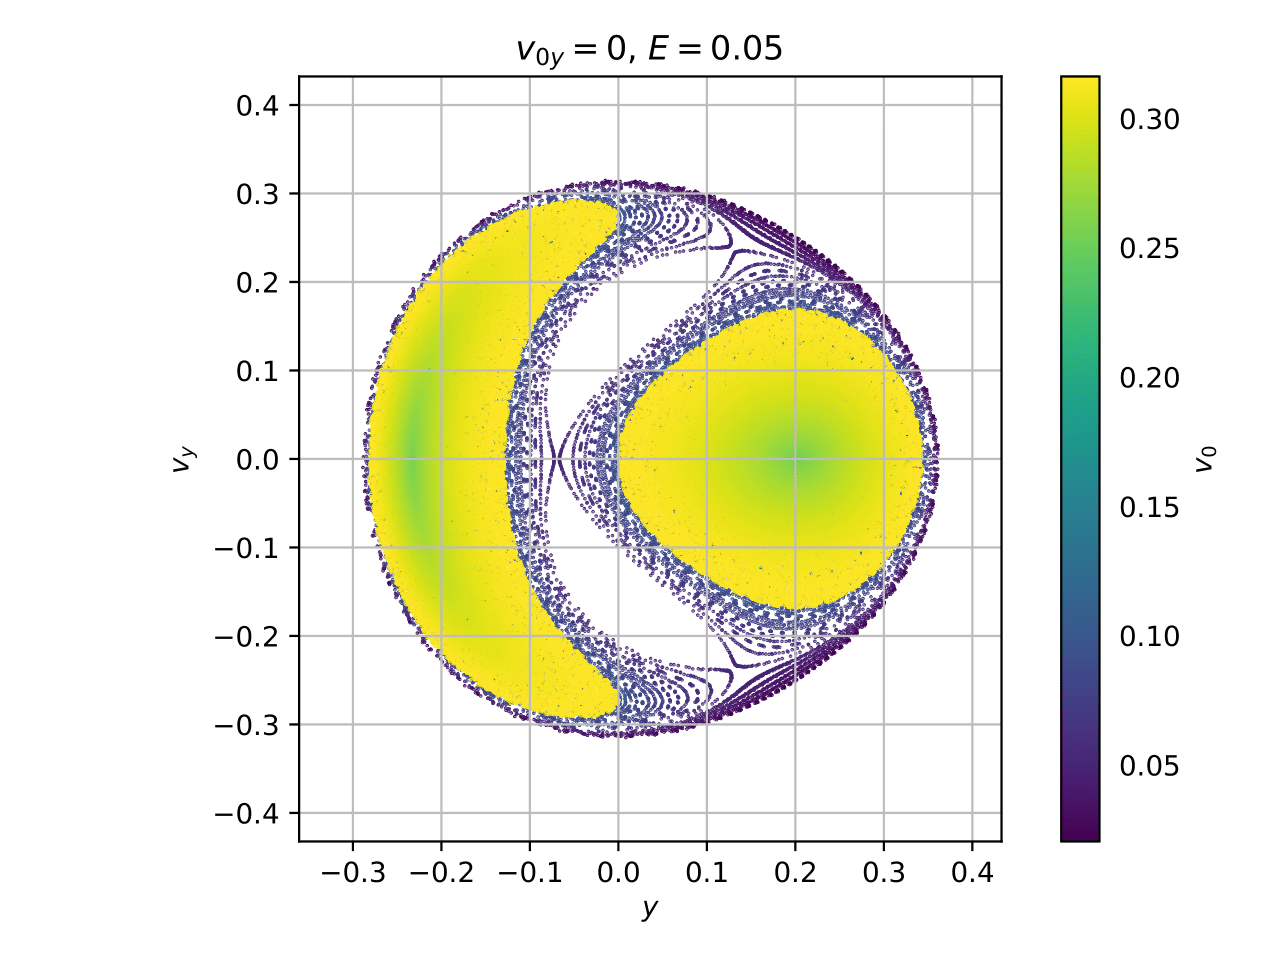
\includegraphics[width=\linewidth]{2.nal_slike/le_v0x/poincare_v0x_E0.05-1.png}
    \end{subfigure}
    \begin{subfigure}{0.49\textwidth}
        \centering
        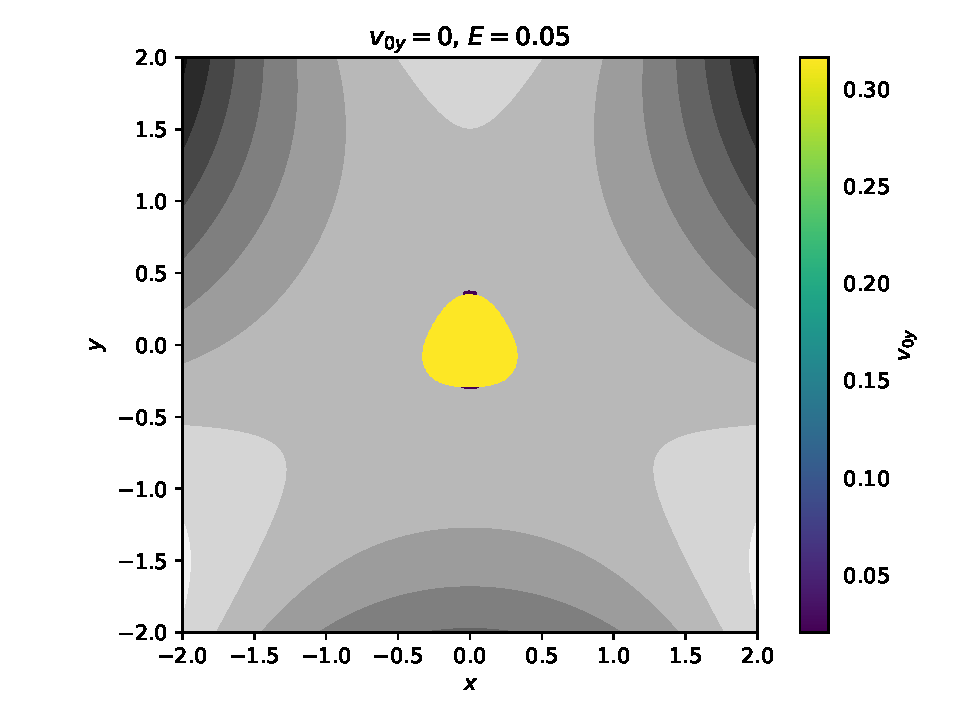
\includegraphics[width=\linewidth]{2.nal_slike/le_v0x/poincare_tajektorije_v0y_E0.05.pdf}
    \end{subfigure}
    \caption{Levo Poincaréjev presek, desno trajktorije pri $E=0,05$}
\end{figure}

\begin{figure}[H]
    \centering
    \begin{subfigure}{0.49\textwidth}
        \centering
        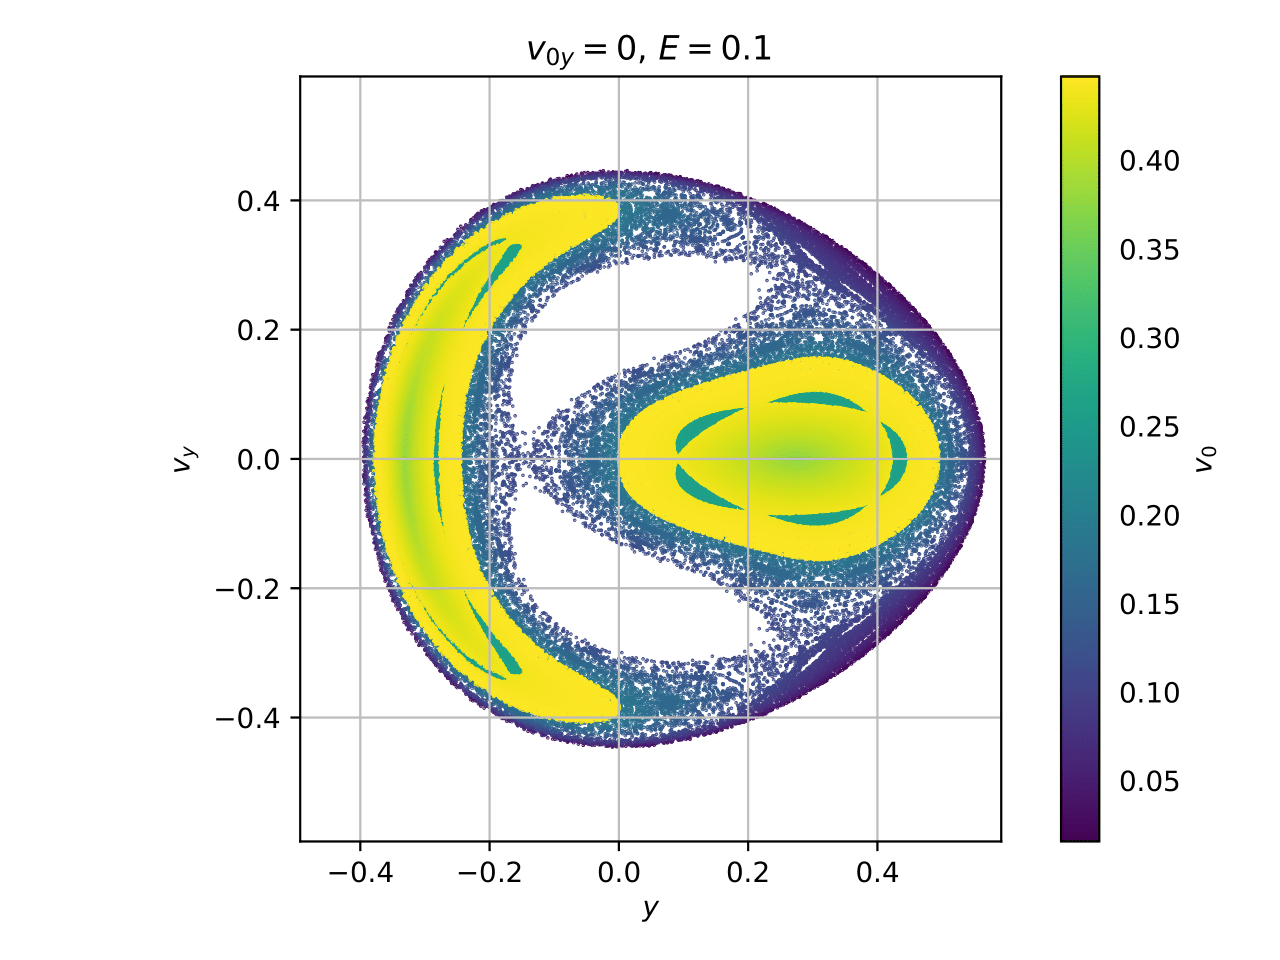
\includegraphics[width=\linewidth]{2.nal_slike/le_v0x/poincare_v0x_E0.1-1.png}
    \end{subfigure}
    \begin{subfigure}{0.49\textwidth}
        \centering
        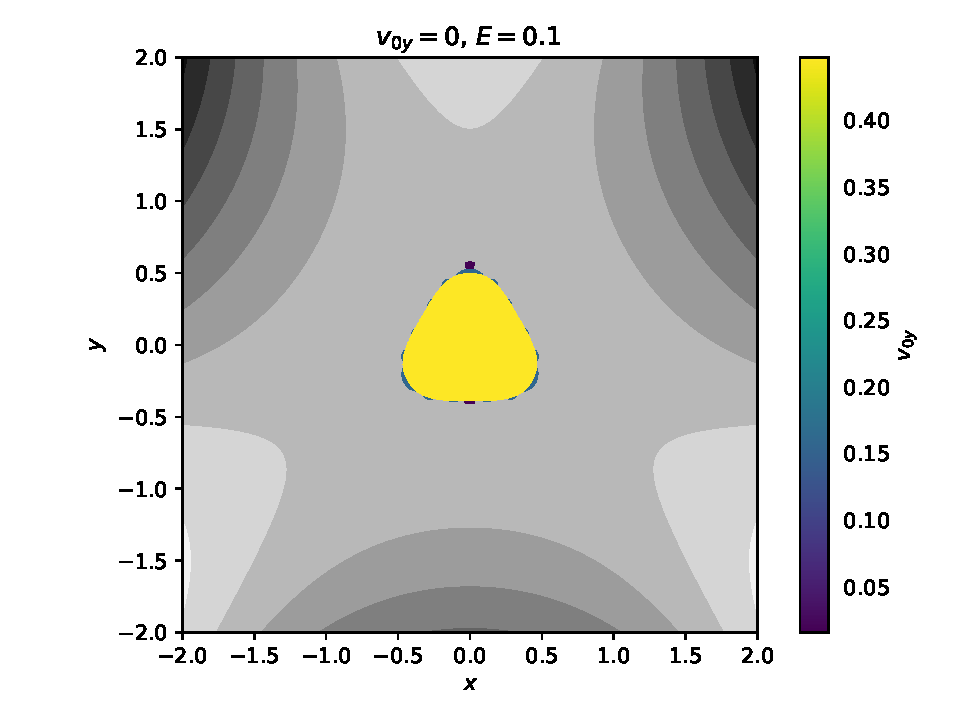
\includegraphics[width=\linewidth]{2.nal_slike/le_v0x/poincare_tajektorije_v0y_E0.1.pdf}
    \end{subfigure}
    \caption{Levo Poincaréjev presek, desno trajktorije pri $E=0,1$}
\end{figure}

\begin{figure}[H]
    \centering
    \begin{subfigure}{0.49\textwidth}
        \centering
        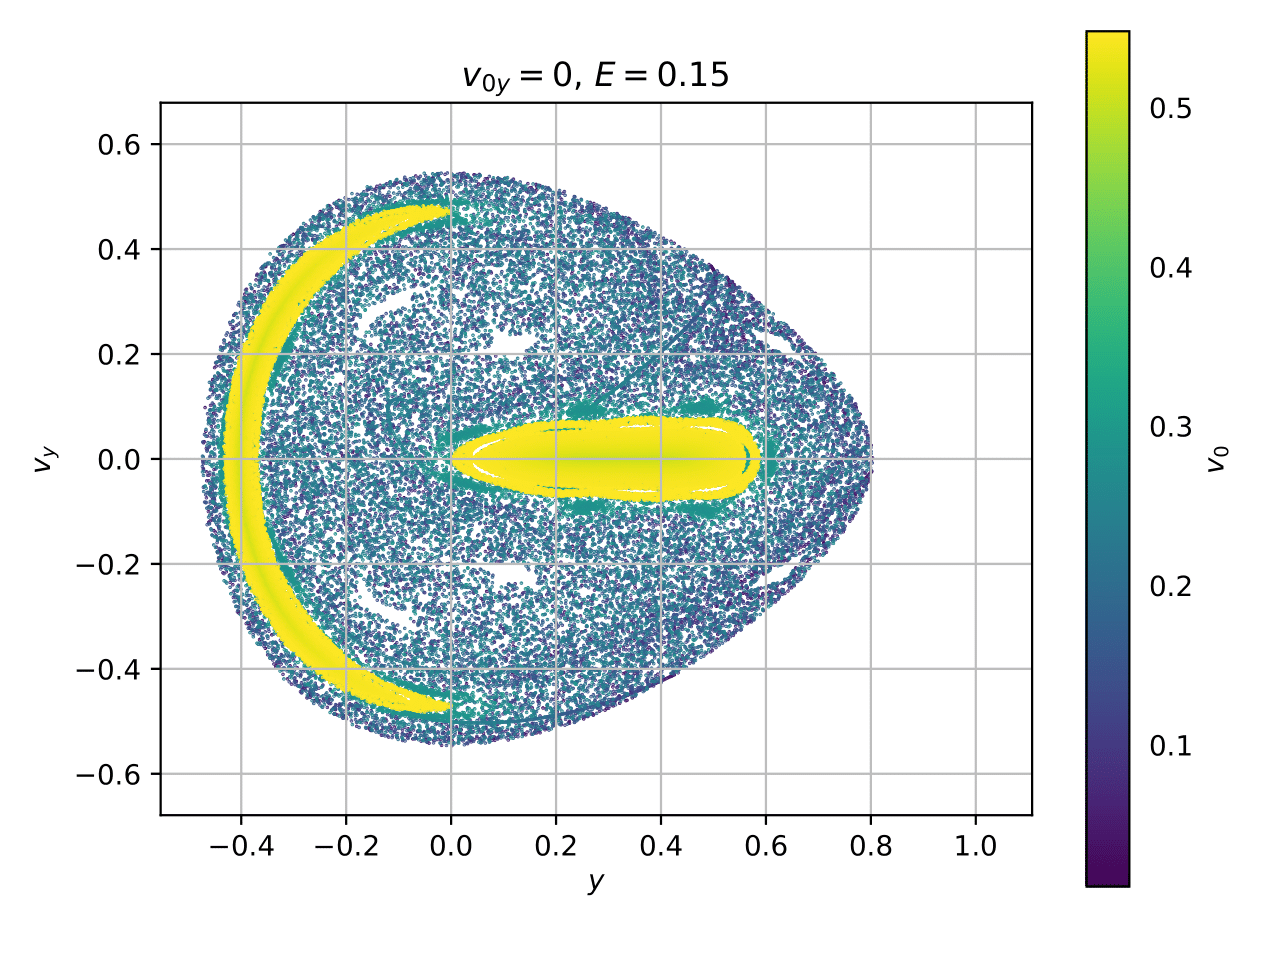
\includegraphics[width=\linewidth]{2.nal_slike/le_v0x/poincare_v0x_E0.15-1.png}
    \end{subfigure}
    \begin{subfigure}{0.49\textwidth}
        \centering
        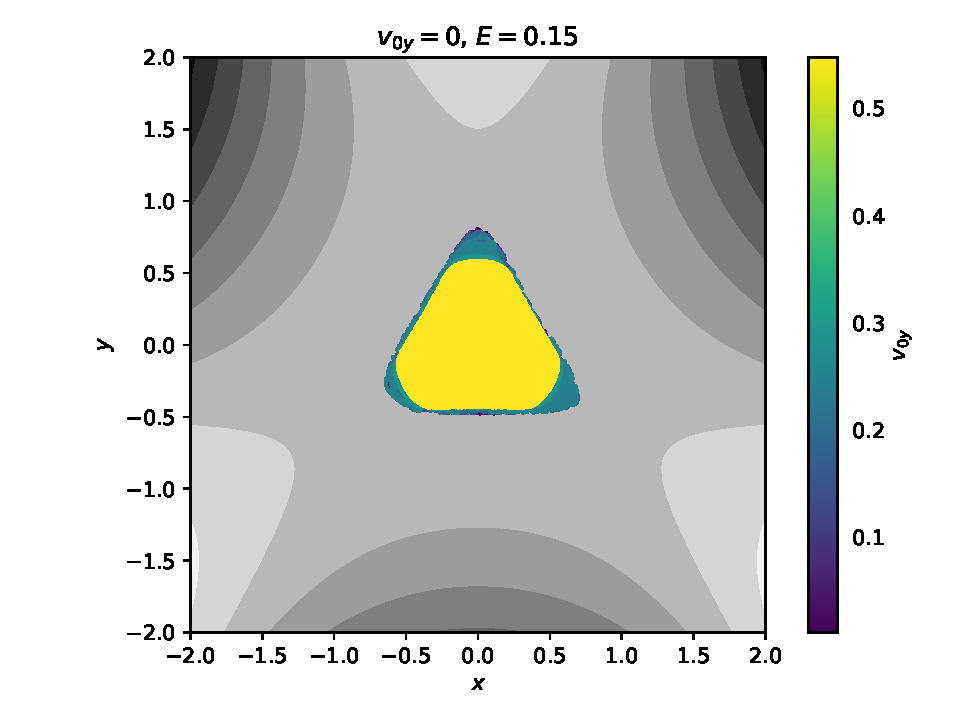
\includegraphics[width=\linewidth]{2.nal_slike/le_v0x/poincare_tajektorije_v0y_E0.15.pdf}
    \end{subfigure}
    \caption{Levo Poincaréjev presek, desno trajktorije pri $E=0,15$}
\end{figure}

\begin{figure}[H]
    \centering
    \begin{subfigure}{0.49\textwidth}
        \centering
        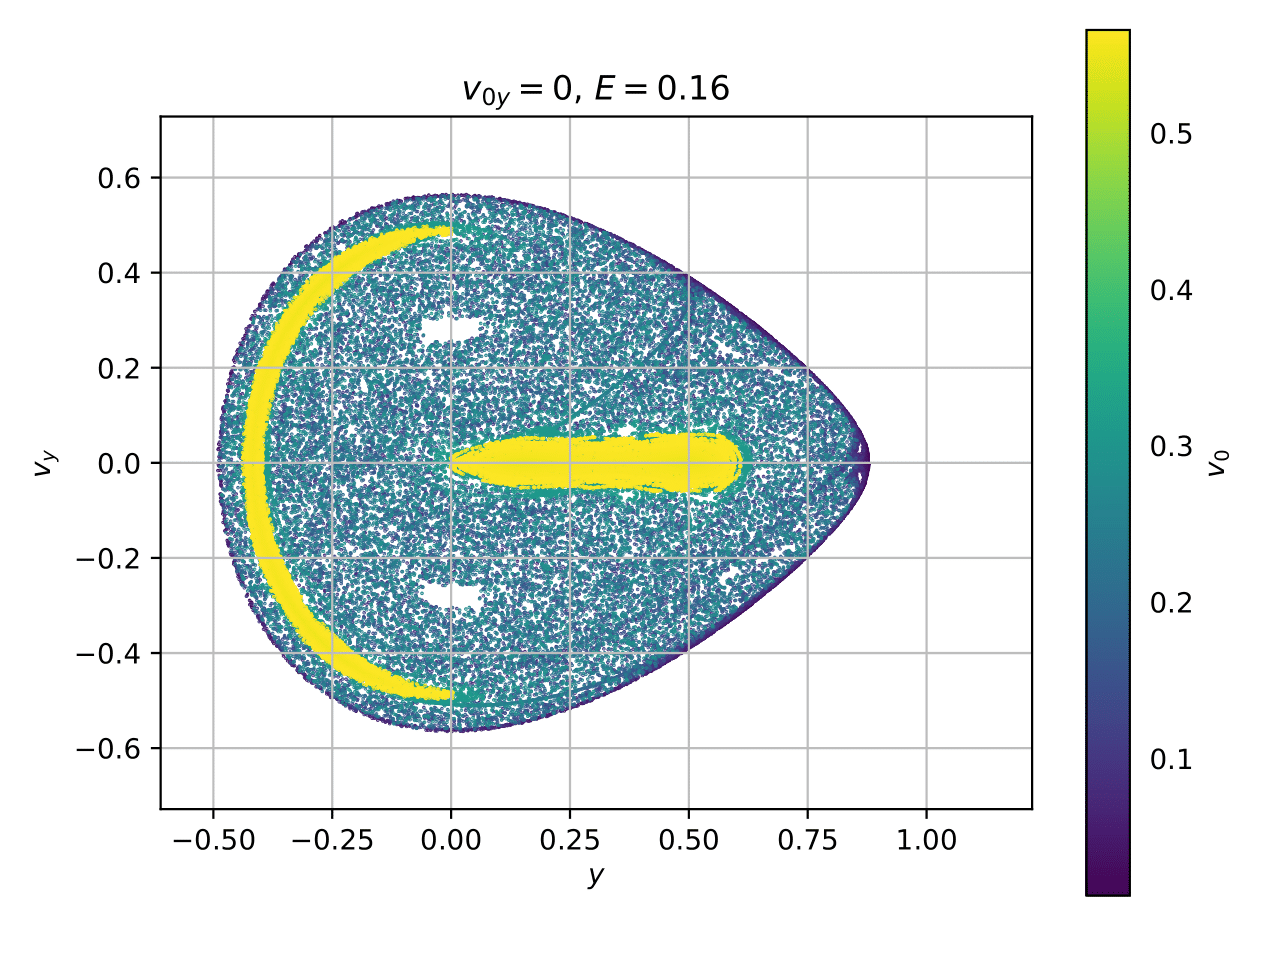
\includegraphics[width=\linewidth]{2.nal_slike/le_v0x/poincare_v0x_E0.16-1.png}
    \end{subfigure}
    \begin{subfigure}{0.49\textwidth}
        \centering
        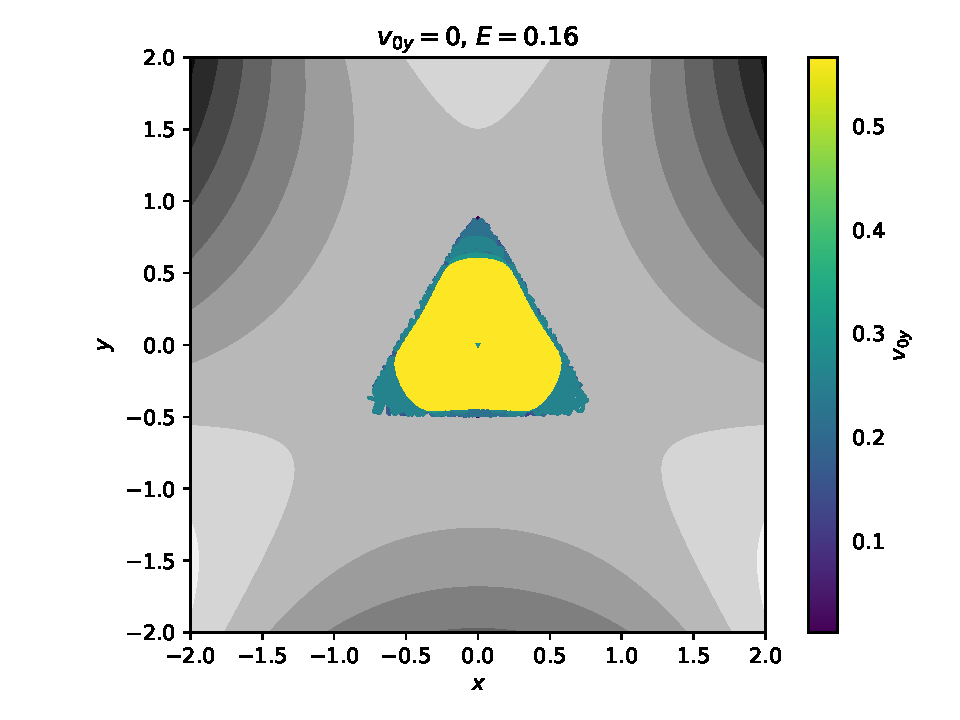
\includegraphics[width=\linewidth]{2.nal_slike/le_v0x/poincare_tajektorije_v0y_E0.16.pdf}
    \end{subfigure}
    \caption{Levo Poincaréjev presek, desno trajktorije pri $E=0,16$}
\end{figure}

\begin{figure}[H]
    \centering
    \begin{subfigure}{0.49\textwidth}
        \centering
        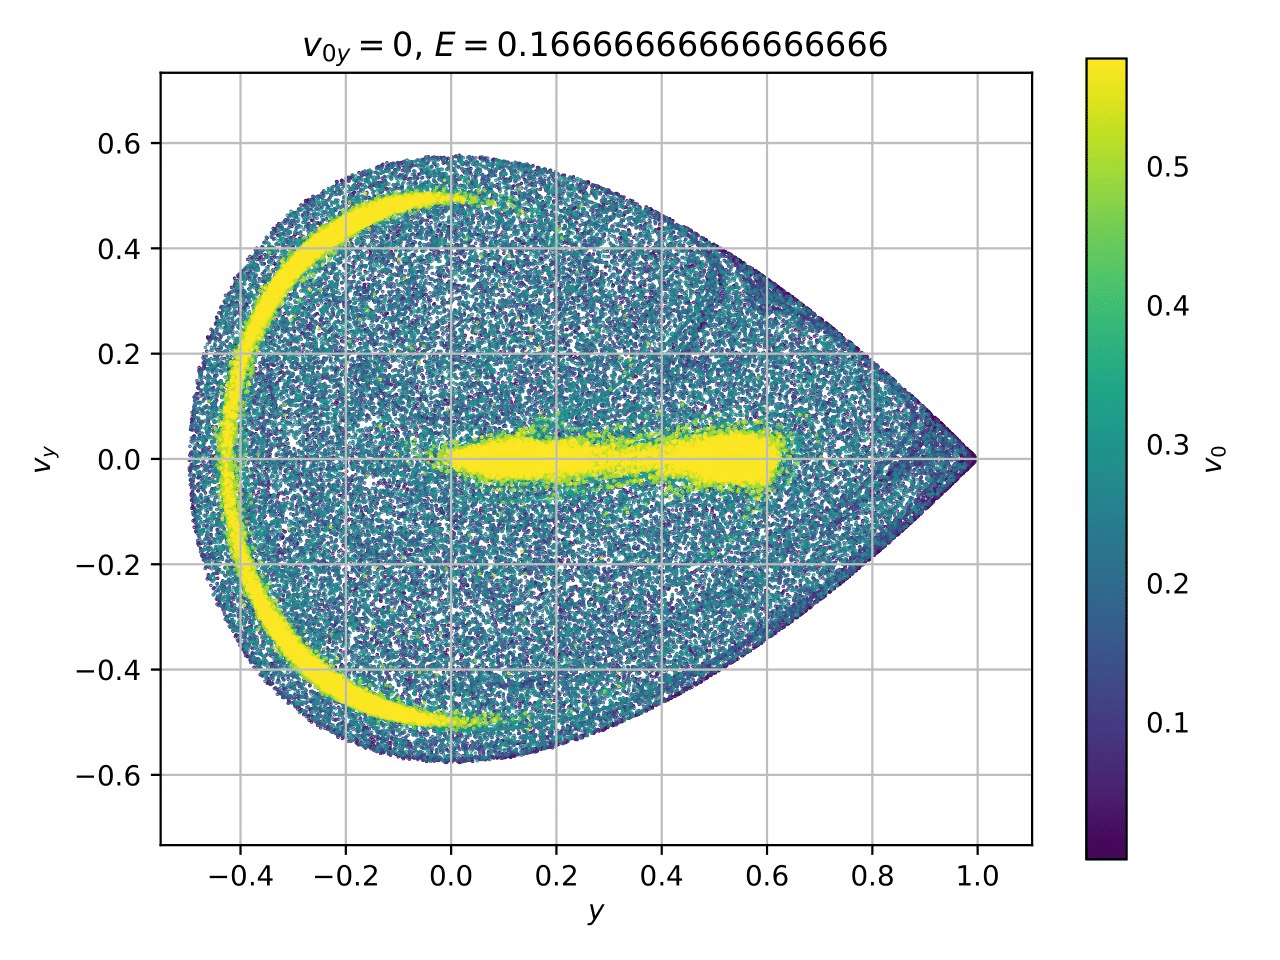
\includegraphics[width=\linewidth]{2.nal_slike/le_v0x/poincare_v0x_E0.16666666666666666-1.png}
    \end{subfigure}
    \begin{subfigure}{0.49\textwidth}
        \centering
        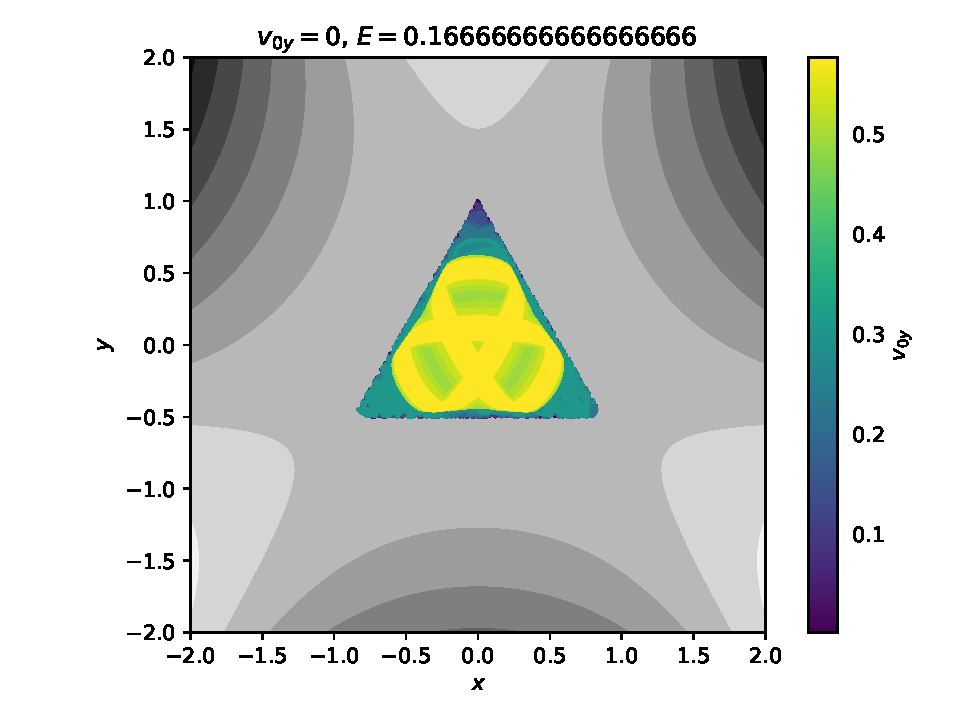
\includegraphics[width=\linewidth]{2.nal_slike/le_v0x/poincare_tajektorije_v0y_E0.16666666666666666.pdf}
    \end{subfigure}
    \caption{Levo Poincaréjev presek, desno trajktorije pri $E=1/6$}
\end{figure}

\begin{figure}[H]
    \centering
    \begin{subfigure}{0.49\textwidth}
        \centering
        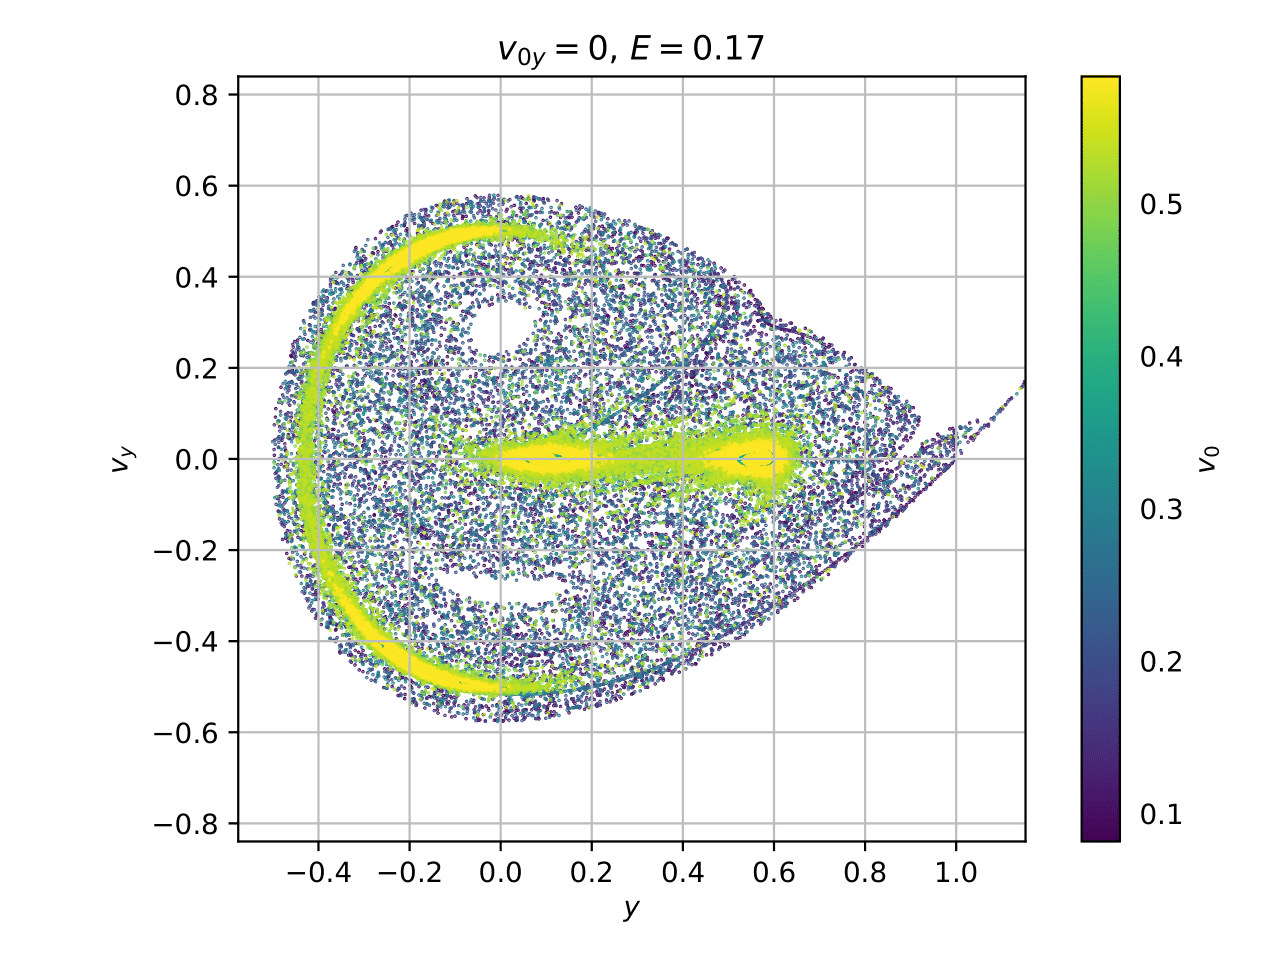
\includegraphics[width=\linewidth]{2.nal_slike/le_v0x/poincare_v0x_E0.17-1.png}
    \end{subfigure}
    \begin{subfigure}{0.49\textwidth}
        \centering
        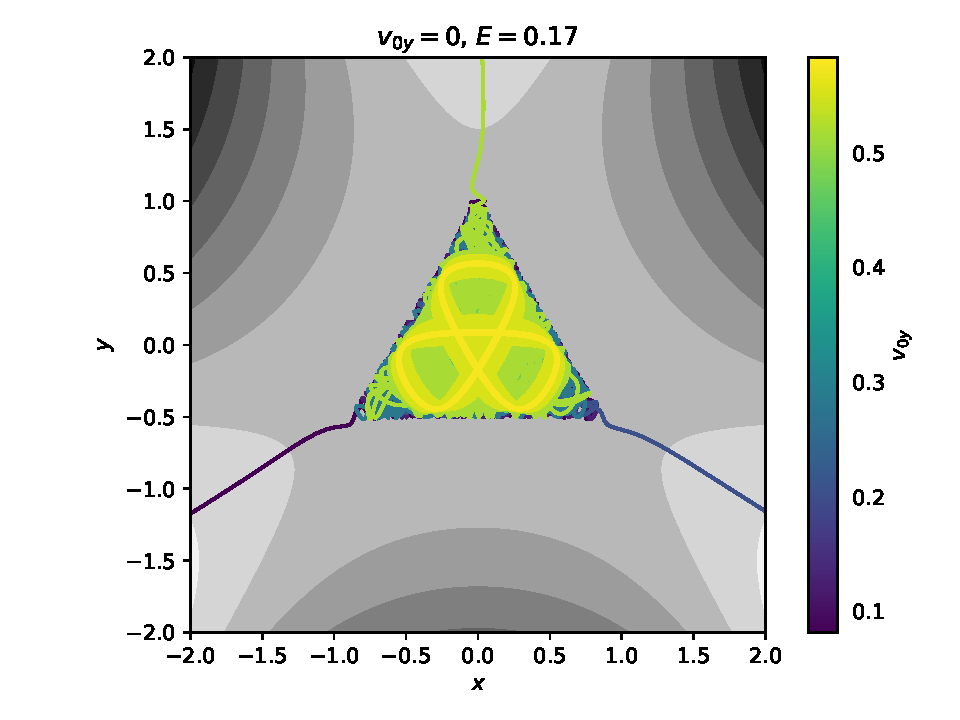
\includegraphics[width=\linewidth]{2.nal_slike/le_v0x/poincare_tajektorije_v0y_E0.17.pdf}
    \end{subfigure}
    \caption{Levo Poincaréjev presek, desno trajktorije pri $E=0,17$}
\end{figure}

\begin{figure}[H]
    \centering
    \begin{subfigure}{0.49\textwidth}
        \centering
        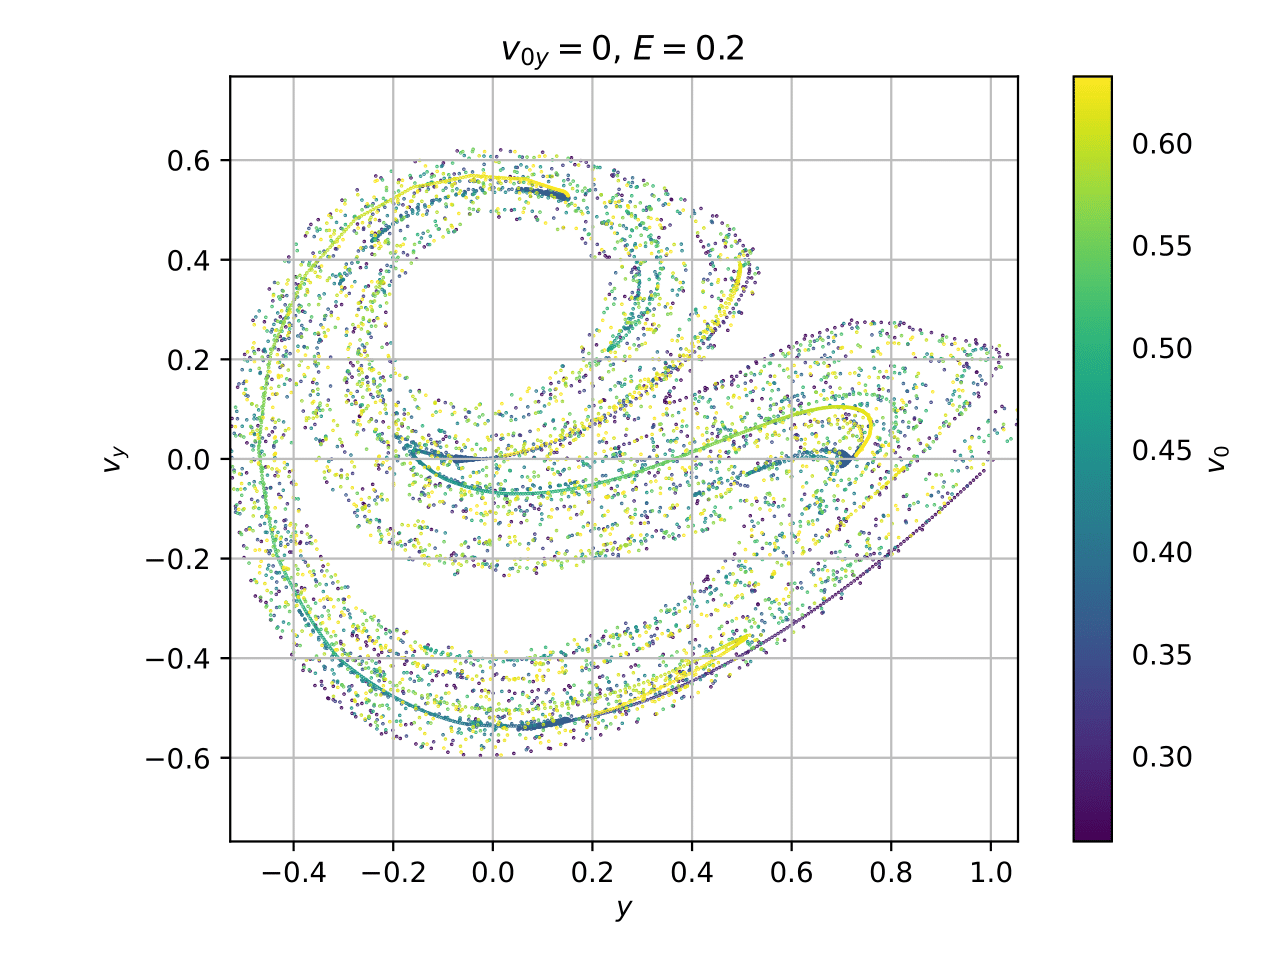
\includegraphics[width=\linewidth]{2.nal_slike/le_v0x/poincare_v0x_E0.2-1.png}
    \end{subfigure}
    \begin{subfigure}{0.49\textwidth}
        \centering
        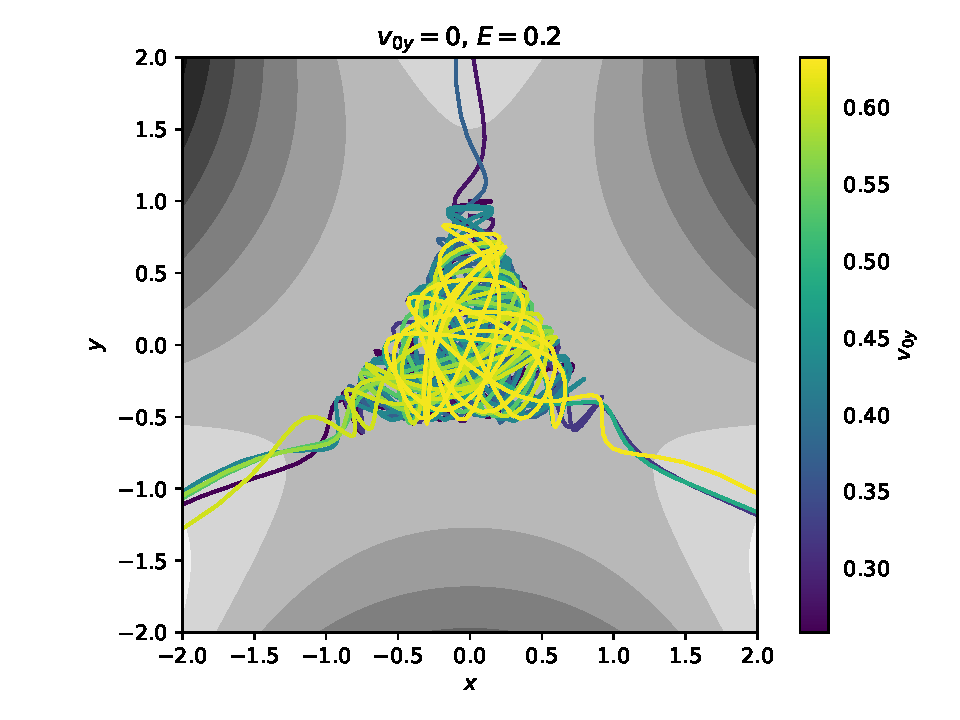
\includegraphics[width=\linewidth]{2.nal_slike/le_v0x/poincare_tajektorije_v0y_E0.2.pdf}
    \end{subfigure}
    \caption{Levo Poincaréjev presek, desno trajktorije pri $E=0,2$}
\end{figure}

Sledi prikaz Poincaréjevih pri $v_{0x}=v_{0y}$ in bolj splošnem gibanju pri poljubnih $y_0$ in $v_{0x}$ med [0,1] ter nato po izrazu za konstantno energijo izračunene $v_{0y}$.

Presenetljivo dobim na tak način precej različne preseke in pri $v_{0x}=v_{0y}$ se periodičnost kmalu izgubi, dočim je v zgornjem primeru prisotna. Zaradi velikosti datoteke sem štedil na kakovosti slik Poincaréjevih presekov, saj je tam prikazanih veliko točk, in so zato prikazane v \textit{png} formatu, le one za splošno hitrost so v \textit{pdf}.

\begin{figure}[h]
    \centering
    \begin{subfigure}{0.49\textwidth}
        \centering
        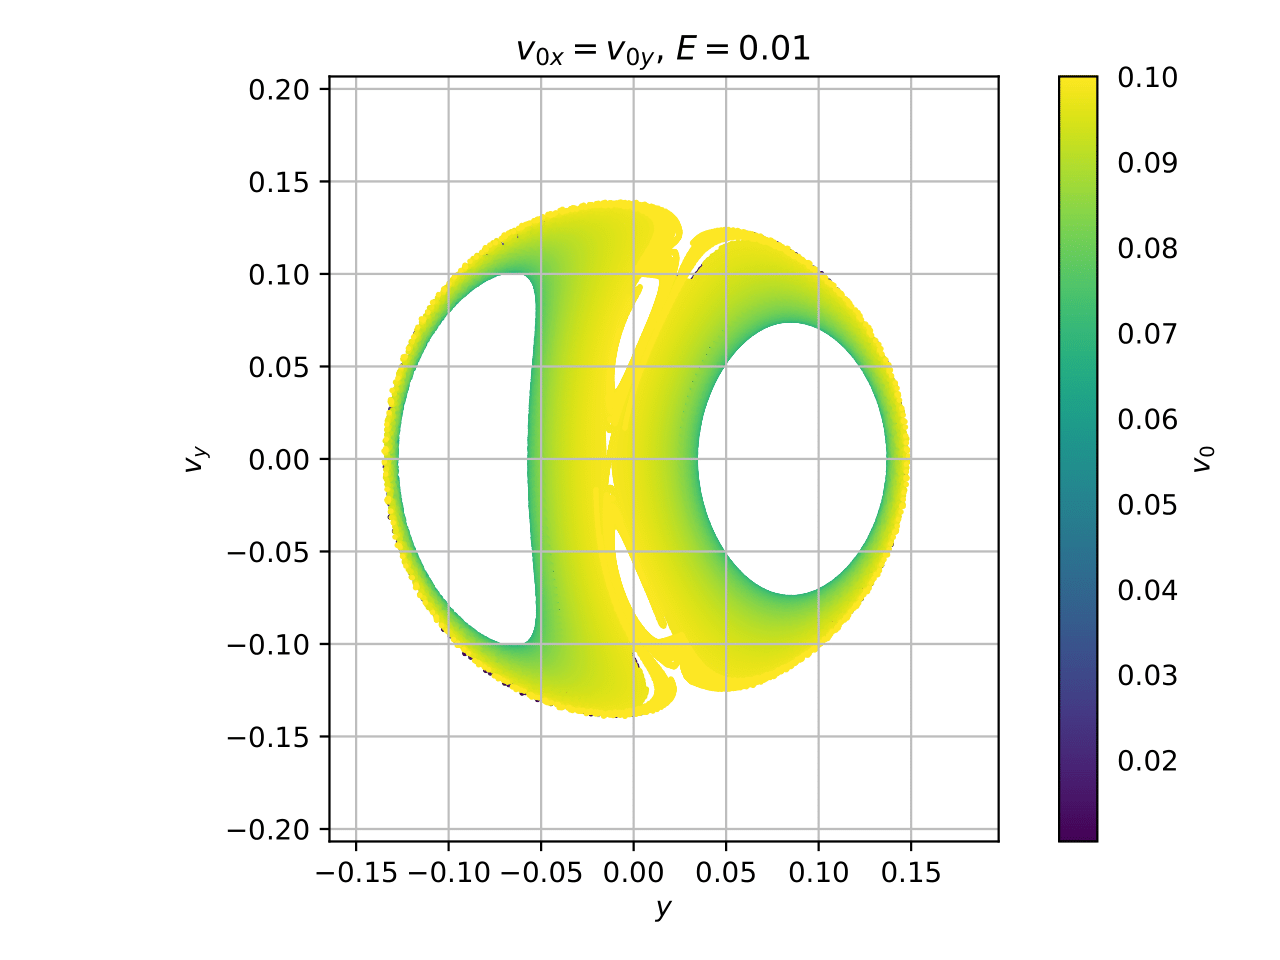
\includegraphics[width=\linewidth]{2.nal_slike/v_0x_enako_v_0y/poincare_v0x_v0y_E0.01-1.png}
    \end{subfigure}
    \begin{subfigure}{0.49\textwidth}
        \centering
        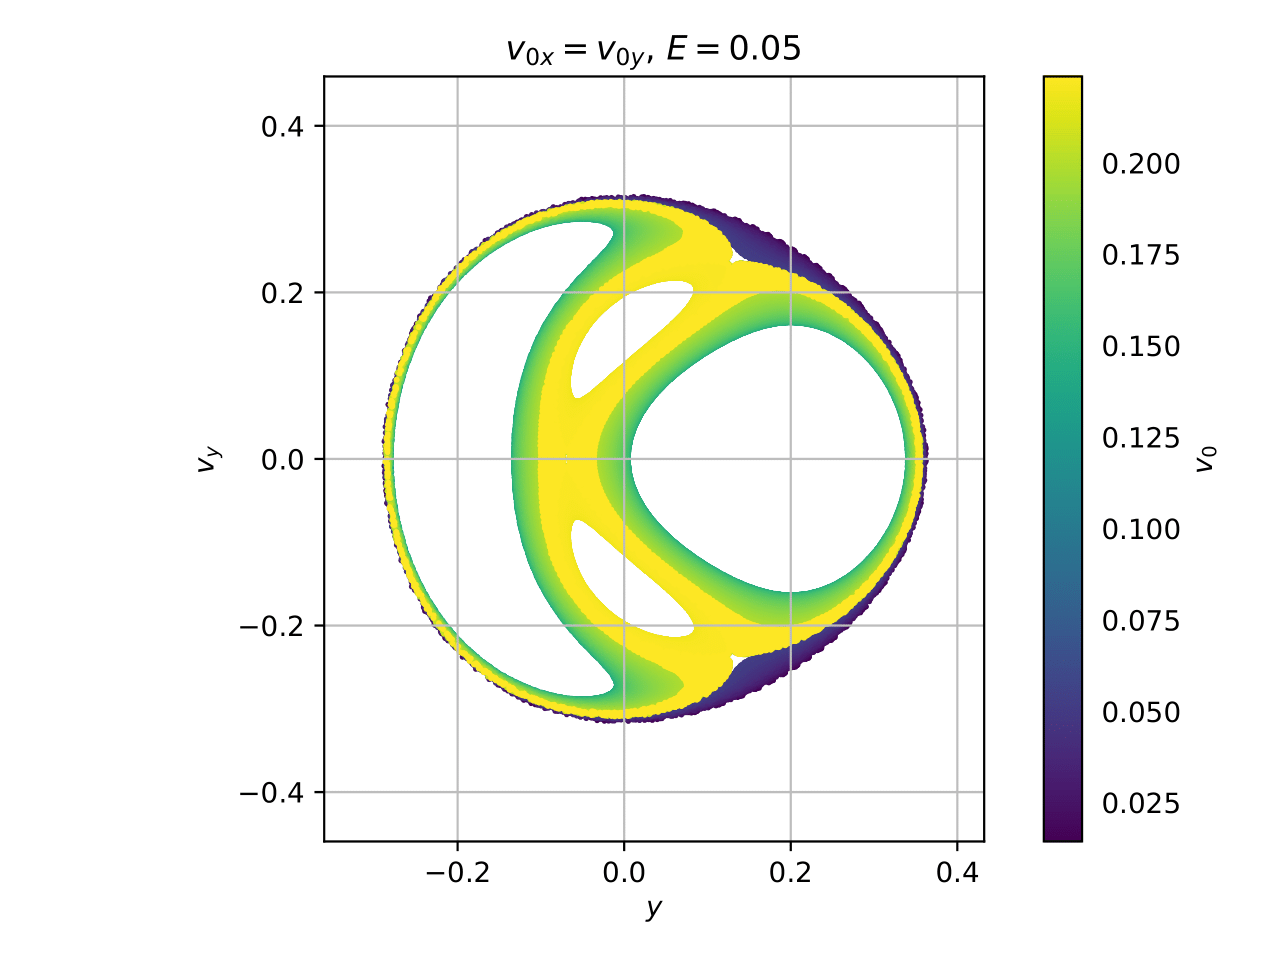
\includegraphics[width=\linewidth]{2.nal_slike/v_0x_enako_v_0y/poincare_v0x_v0y_E0.05-1.png}
    \end{subfigure}
    \begin{subfigure}{0.49\textwidth}
        \centering
        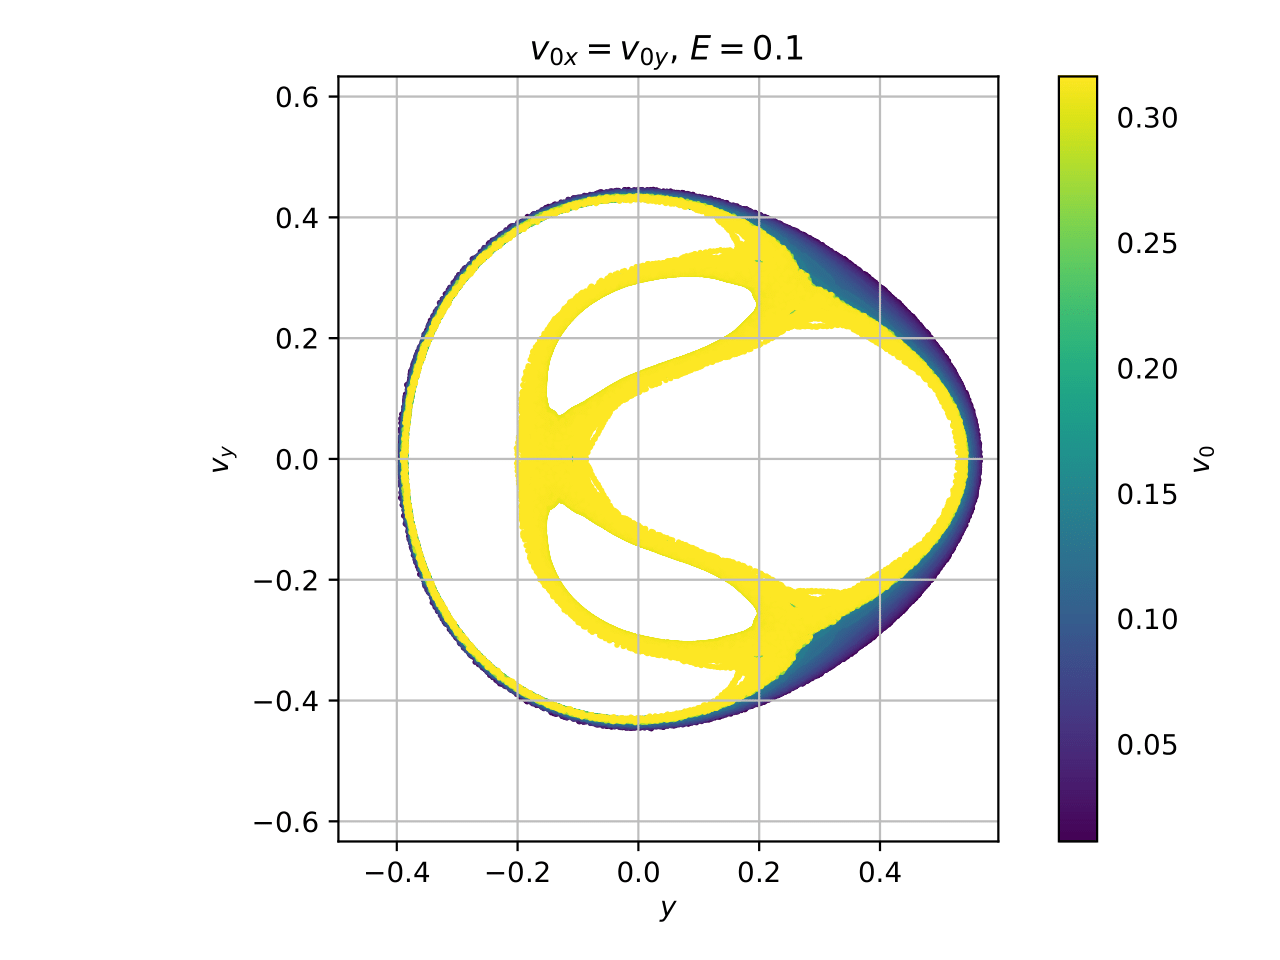
\includegraphics[width=\linewidth]{2.nal_slike/v_0x_enako_v_0y/poincare_v0x_v0y_E0.1-1.png}
    \end{subfigure}
    \begin{subfigure}{0.49\textwidth}
        \centering
        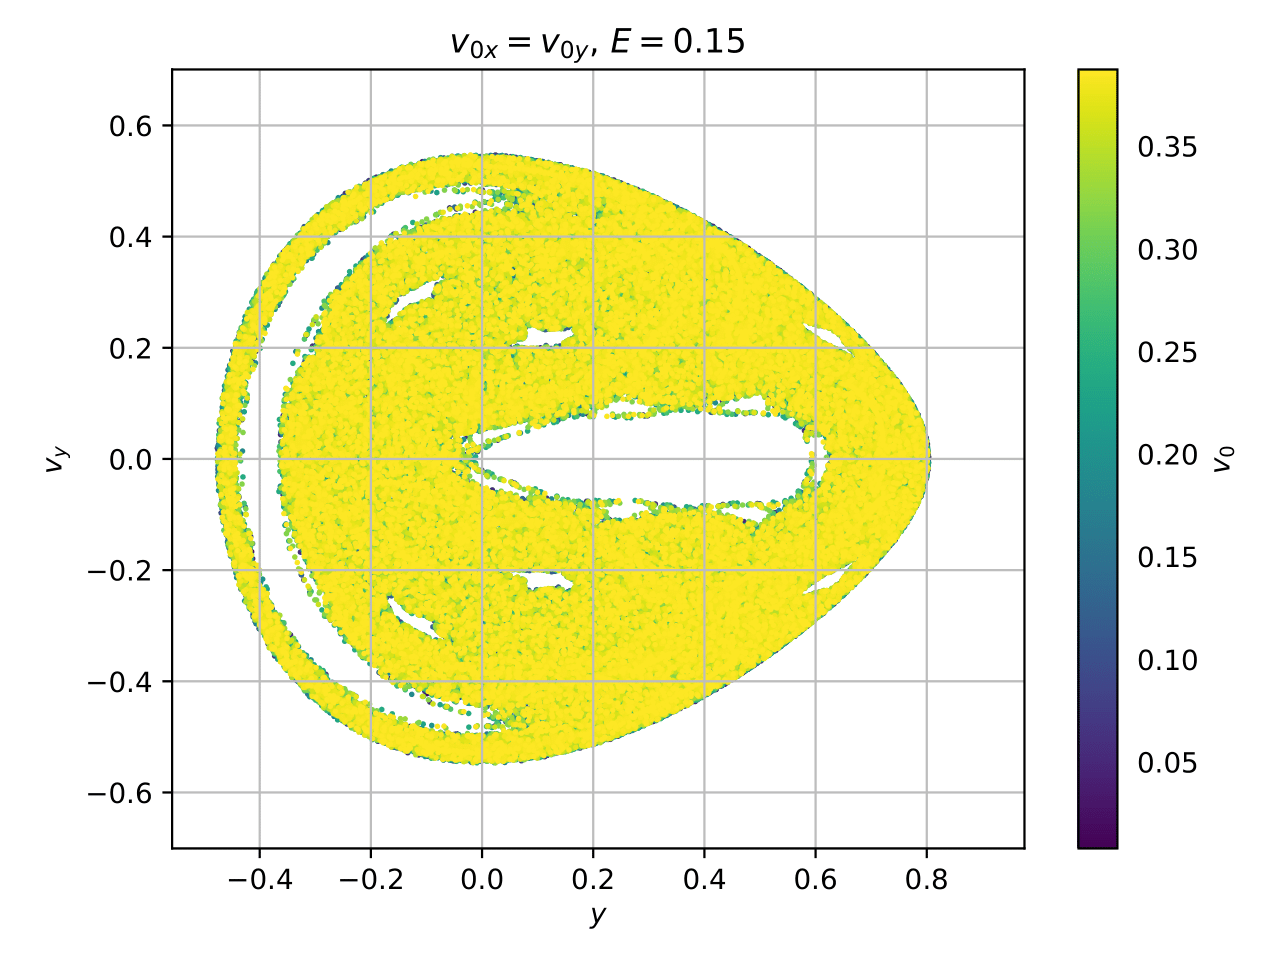
\includegraphics[width=\linewidth]{2.nal_slike/v_0x_enako_v_0y/poincare_v0x_v0y_E0.15-1.png}
    \end{subfigure}
    \begin{subfigure}{0.49\textwidth}
        \centering
        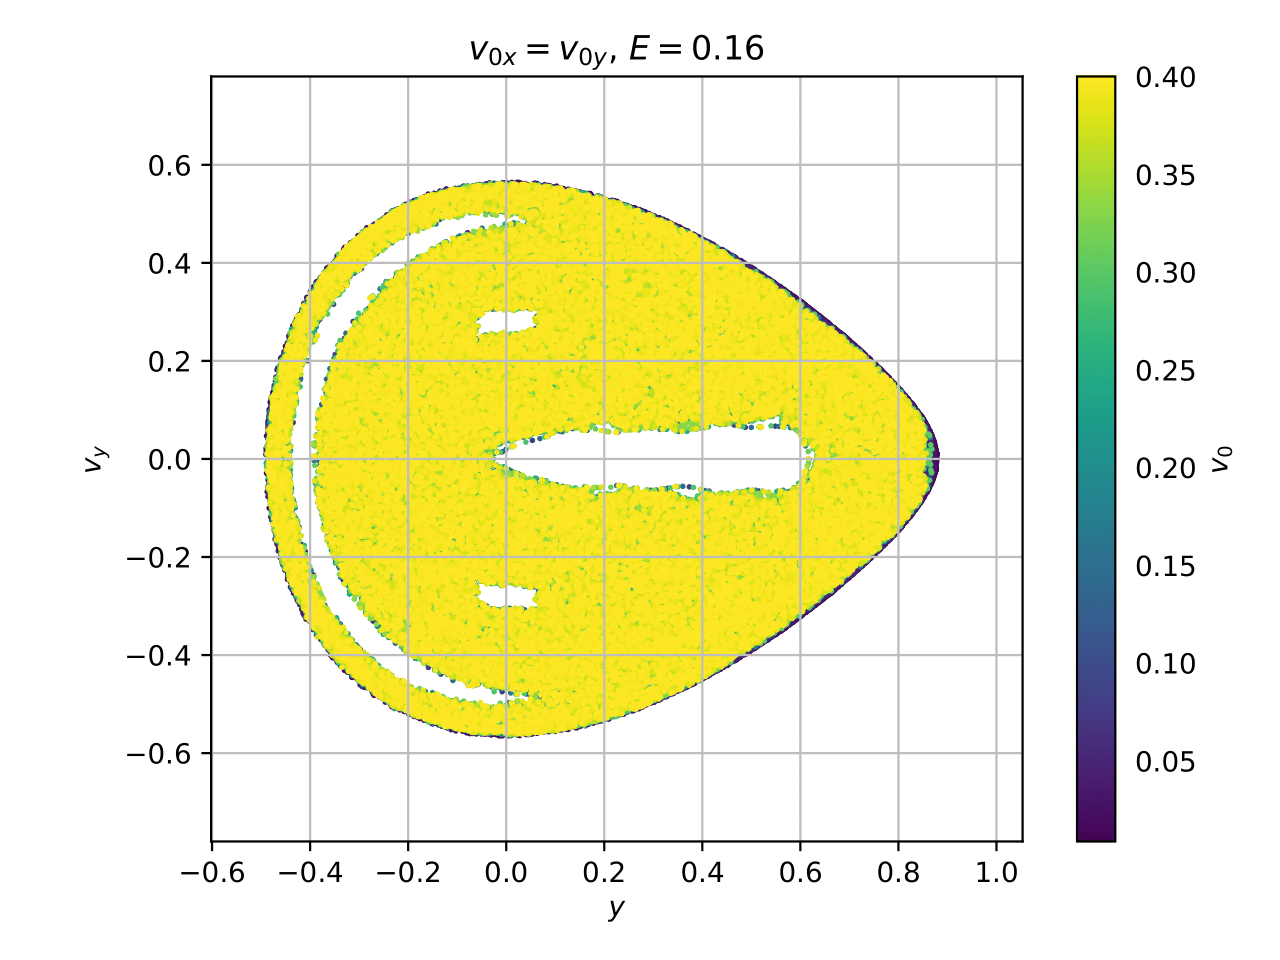
\includegraphics[width=\linewidth]{2.nal_slike/v_0x_enako_v_0y/poincare_v0x_v0y_E0.16-1.png}
    \end{subfigure}
    \begin{subfigure}{0.49\textwidth}
        \centering
        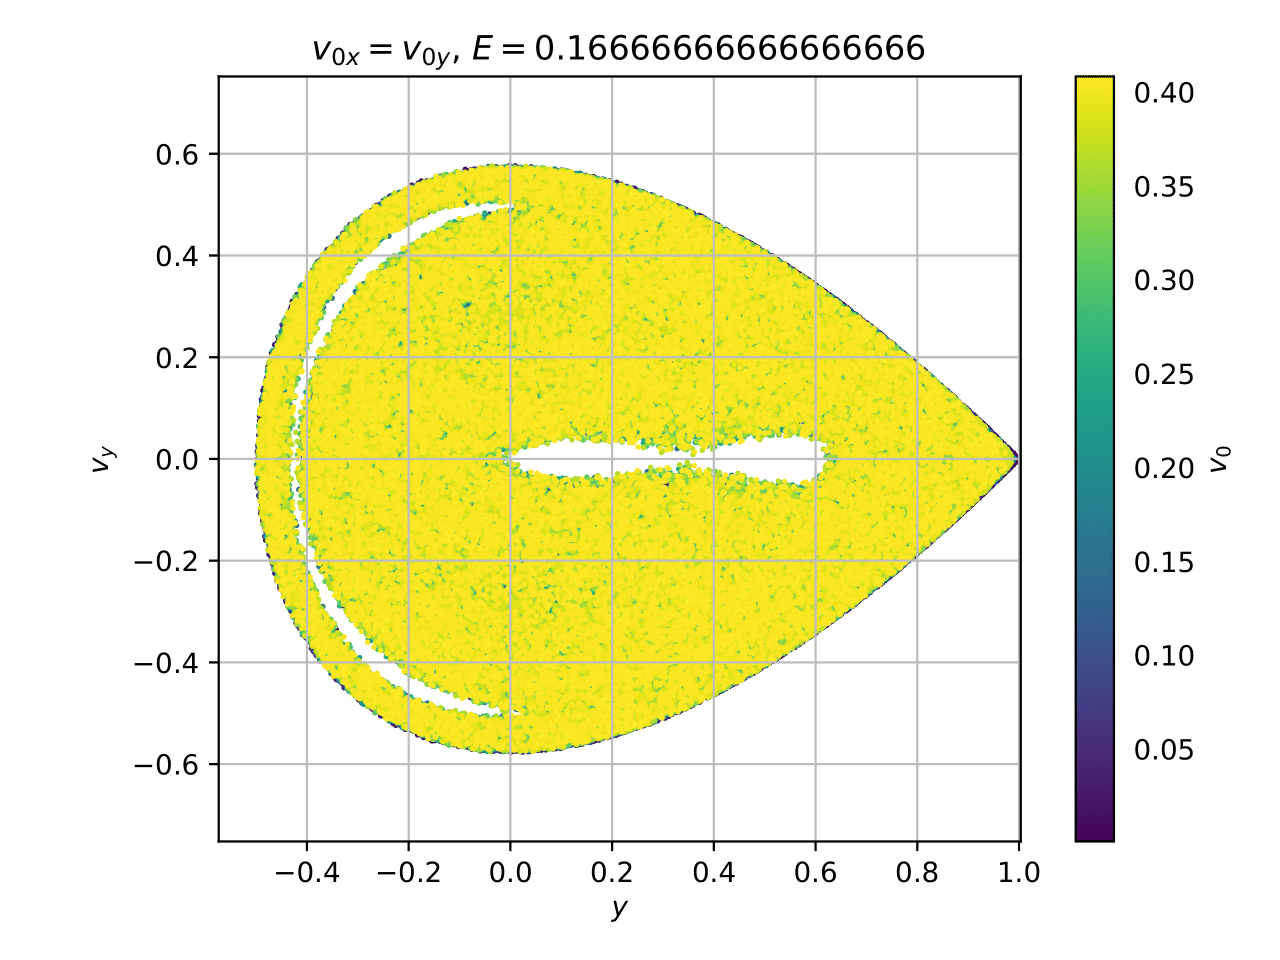
\includegraphics[width=\linewidth]{2.nal_slike/v_0x_enako_v_0y/poincare_v0x_v0y_E0.16666666666666666-1.png}
    \end{subfigure}
    \begin{subfigure}{0.49\textwidth}
        \centering
        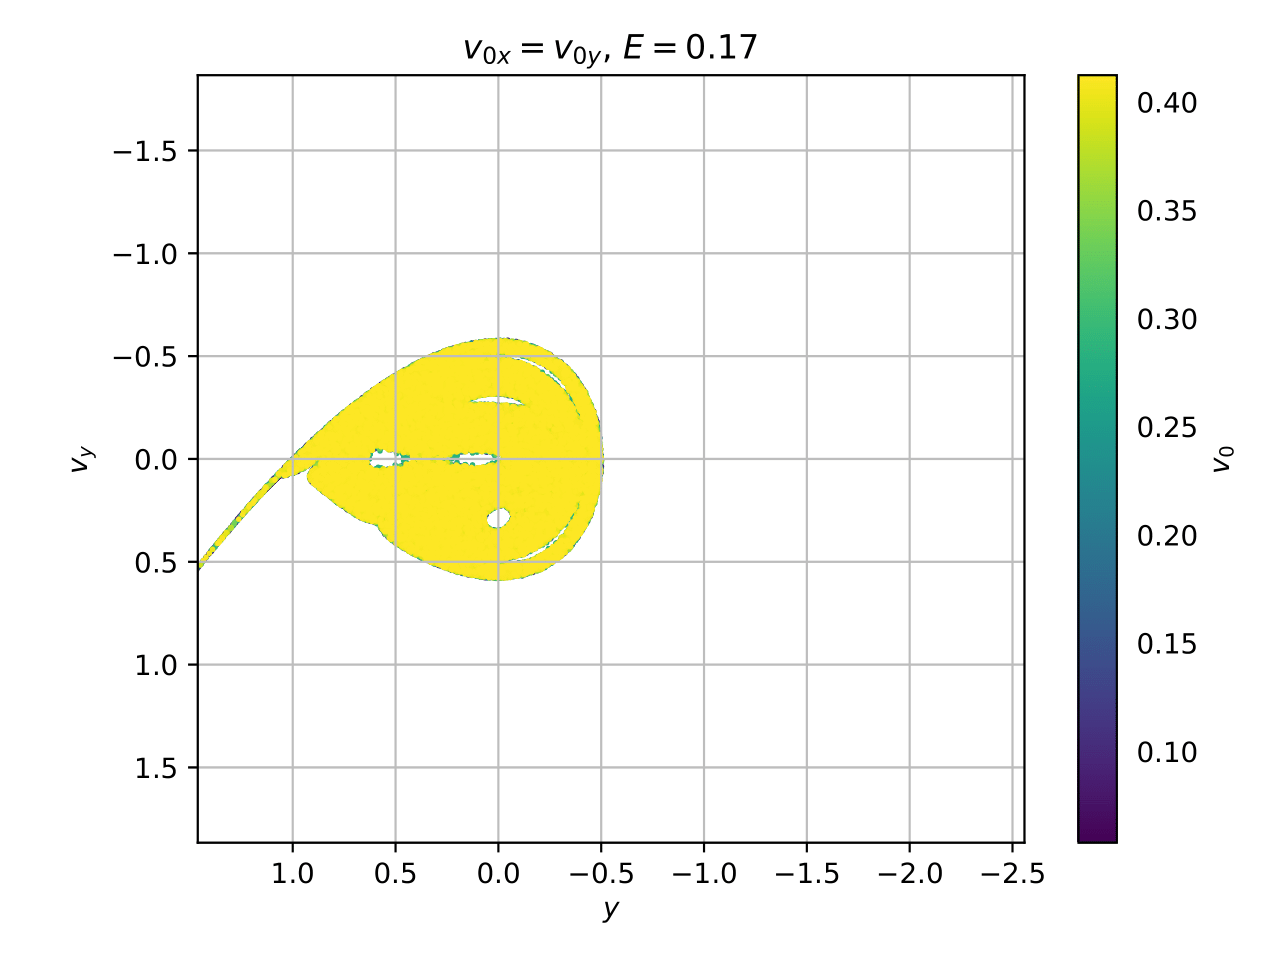
\includegraphics[width=\linewidth]{2.nal_slike/v_0x_enako_v_0y/poincare_v0x_v0y_E0.17-1.png}
    \end{subfigure}
    \begin{subfigure}{0.49\textwidth}
        \centering
        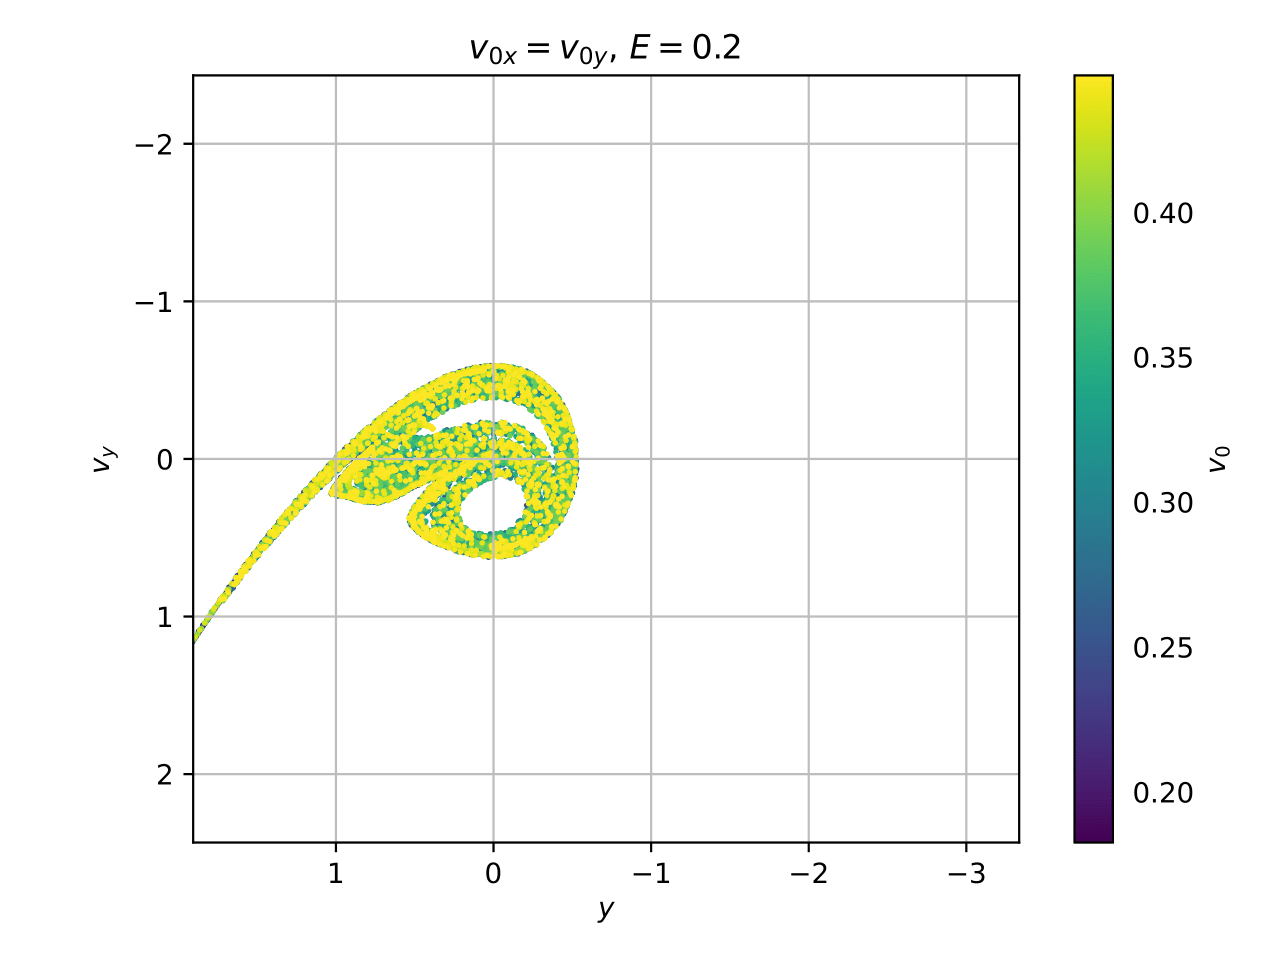
\includegraphics[width=\linewidth]{2.nal_slike/v_0x_enako_v_0y/poincare_v0x_v0y_E0.2-1.png}
    \end{subfigure}
    \caption{Poincaréjevi preseki pri pogoju $v_{x0}=v_{y0}$}
\end{figure}

\begin{figure}[h]
    \centering
    \begin{subfigure}{0.49\textwidth}
        \centering
        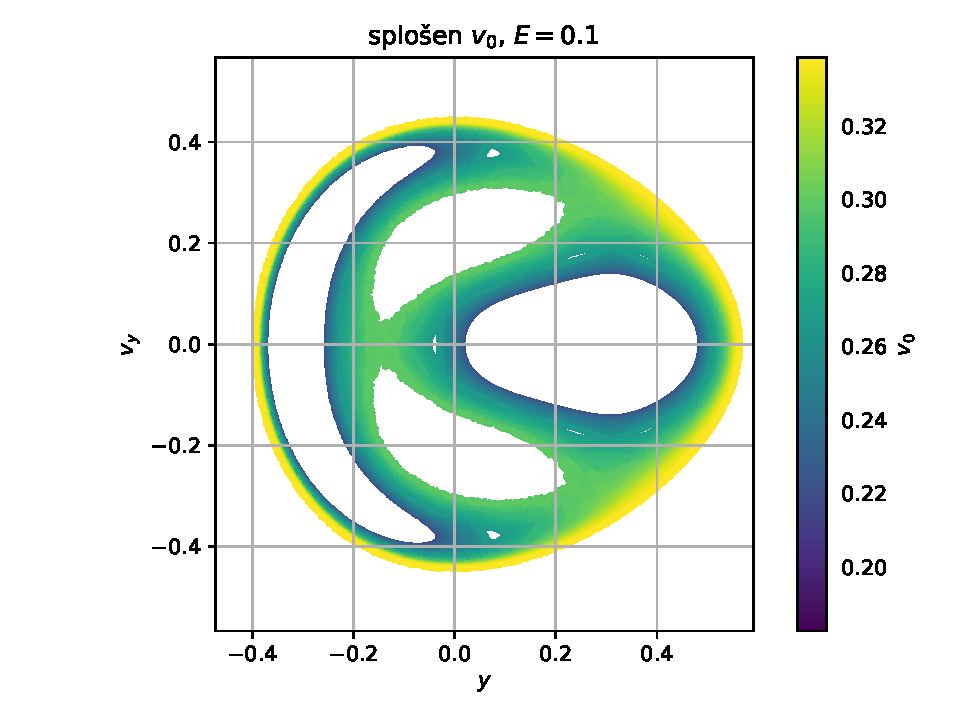
\includegraphics[width=\linewidth]{2.nal_slike/splošen_v0/poincare_v0x_v0y_E0.1.pdf}
    \end{subfigure}
    \begin{subfigure}{0.49\textwidth}
        \centering
        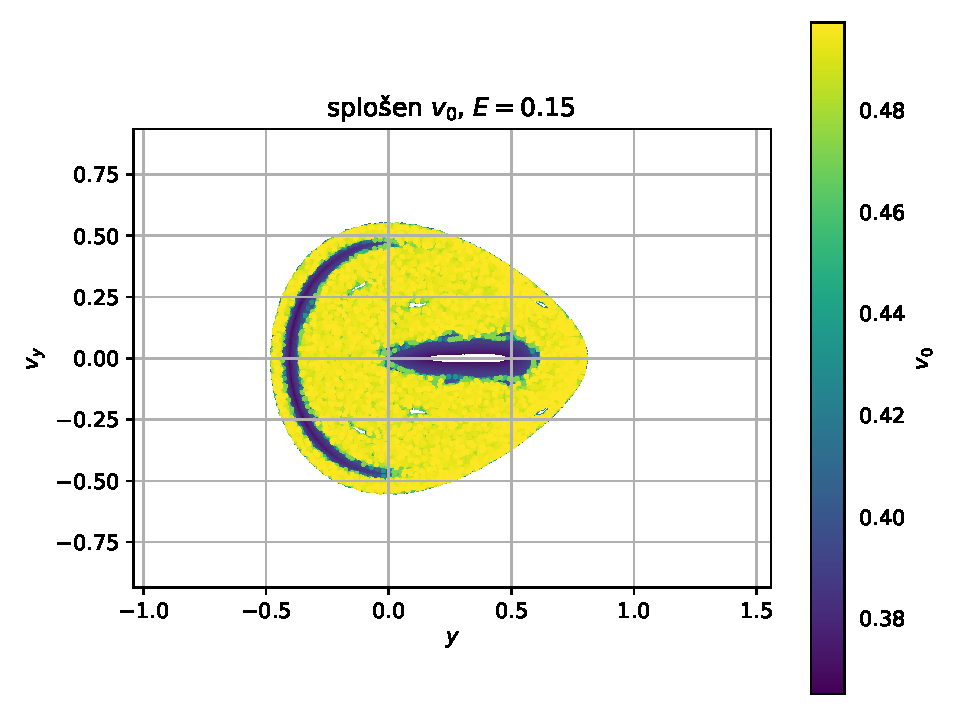
\includegraphics[width=\linewidth]{2.nal_slike/splošen_v0/poincare_v0x_v0y_E0.15.pdf}
    \end{subfigure}
    \begin{subfigure}{0.49\textwidth}
        \centering
        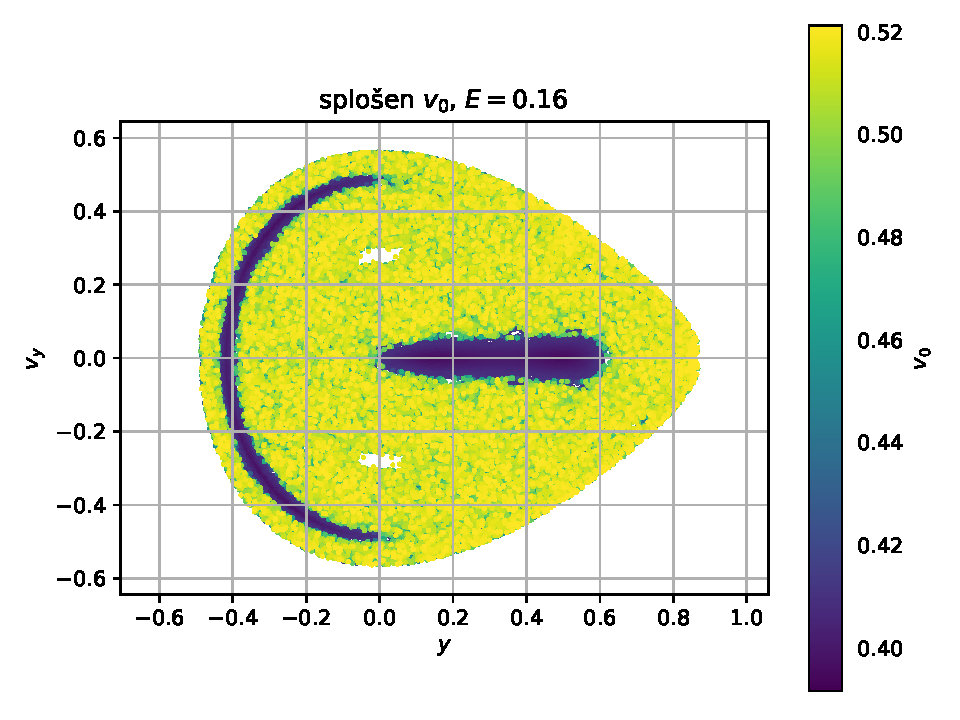
\includegraphics[width=\linewidth]{2.nal_slike/splošen_v0/poincare_v0x_v0y_E0.16.pdf}
    \end{subfigure}
    \begin{subfigure}{0.49\textwidth}
        \centering
        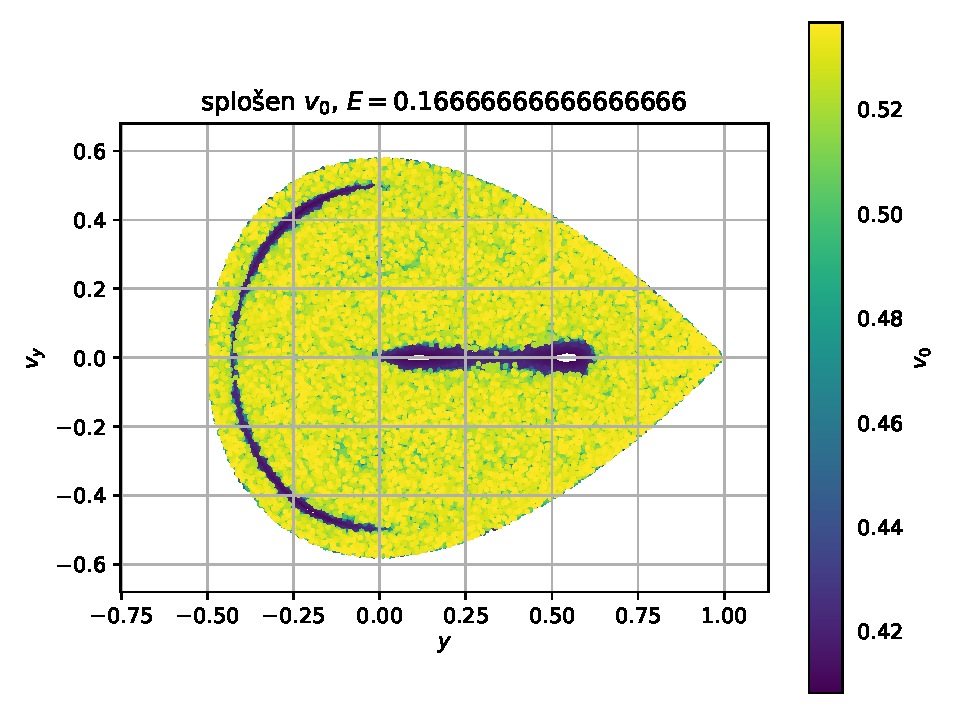
\includegraphics[width=\linewidth]{2.nal_slike/splošen_v0/poincare_v0x_v0y_E0.16666666666666666.pdf}
    \end{subfigure}
    \begin{subfigure}{0.49\textwidth}
        \centering
        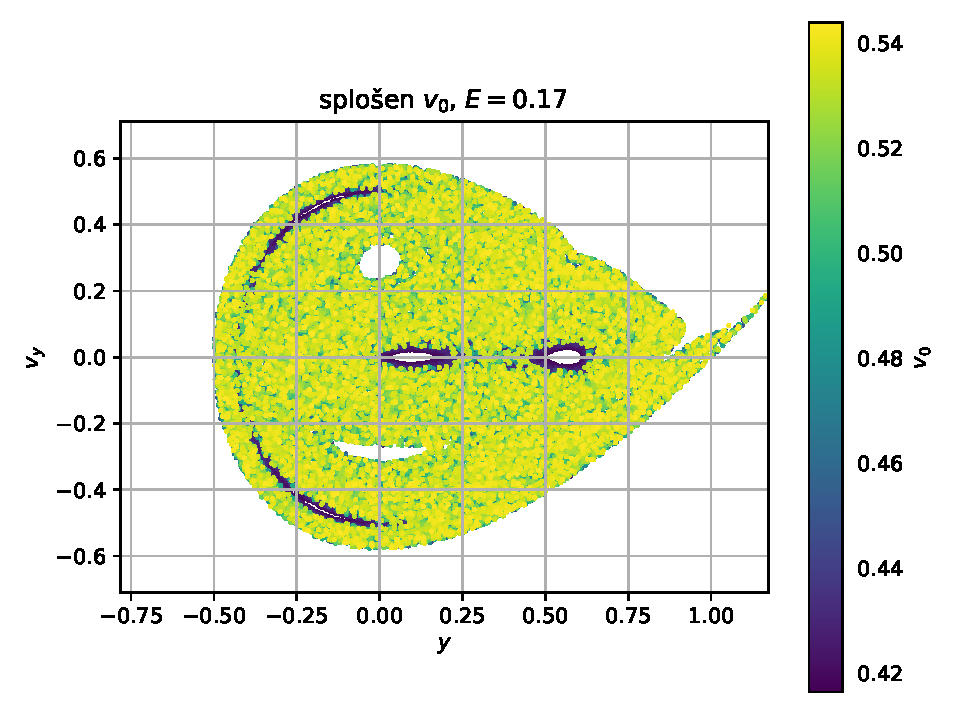
\includegraphics[width=\linewidth]{2.nal_slike/splošen_v0/poincare_v0x_v0y_E0.17.pdf}
    \end{subfigure}
    \begin{subfigure}{0.49\textwidth}
        \centering
        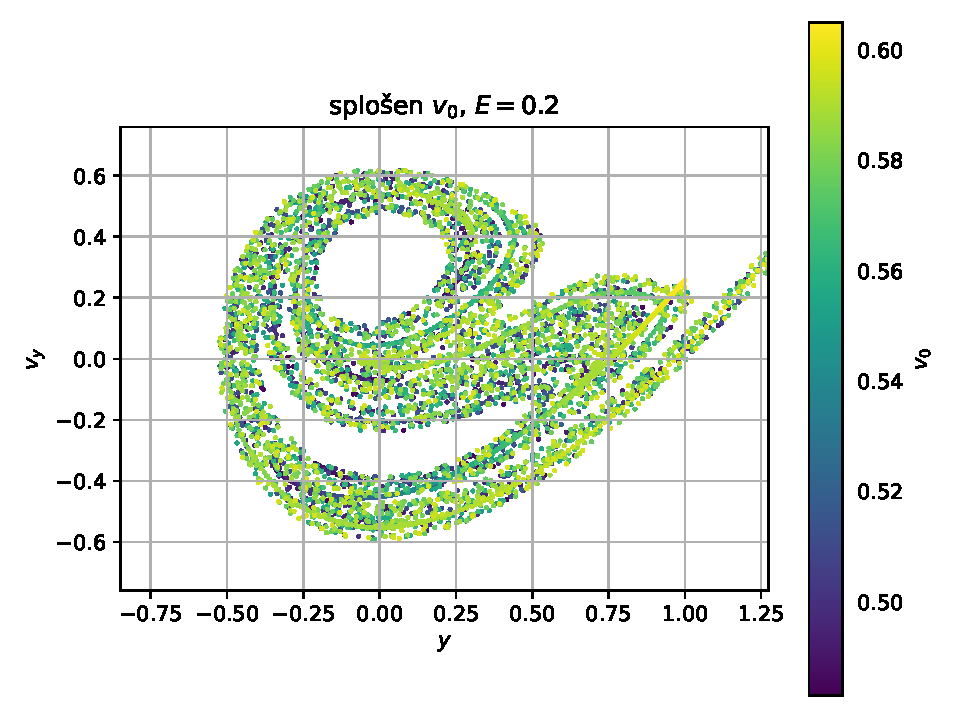
\includegraphics[width=\linewidth]{2.nal_slike/splošen_v0/poincare_v0x_v0y_E0.2.pdf}
    \end{subfigure}
    \caption{Poincaréjevi preseki pri splošnih hitrostih}
\end{figure}

\begin{figure}
    \centering
    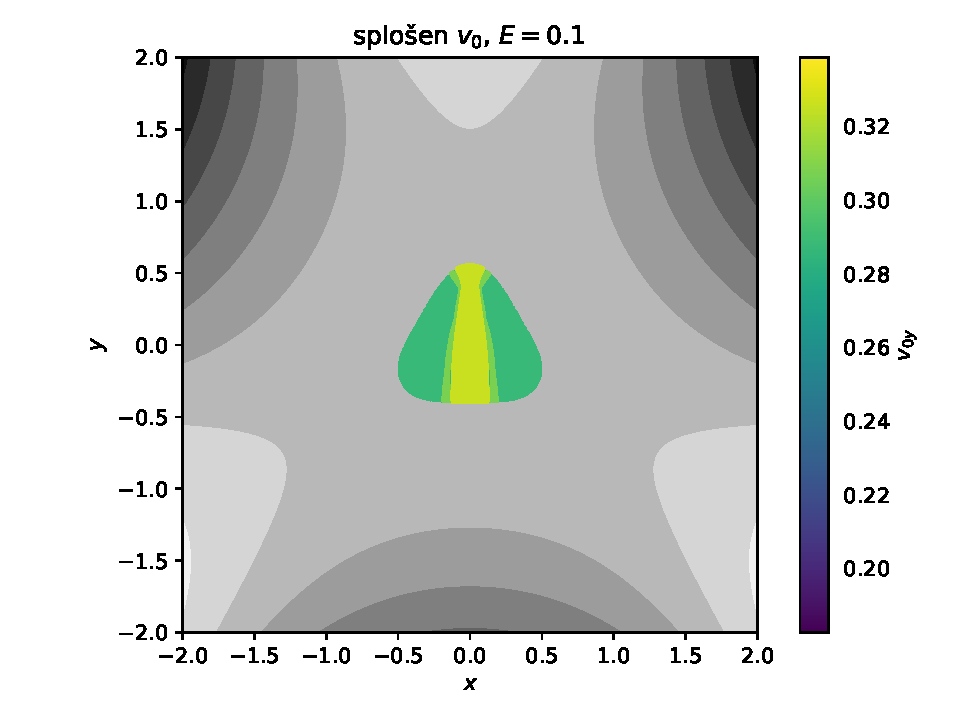
\includegraphics[width=0.6\linewidth]{2.nal_slike/splošen_v0/poincare_tajektorije_v0x_v0y_E0.1.pdf}
    \caption[short]{Zanimive trajektorije pri $E=0,1$ in splošni hitrosti}
\end{figure}